\documentclass[12pt,a4paper]{report}

% ==============================================================================
% Packages & Configuration
% ==============================================================================
\usepackage[utf8]{inputenc}
\usepackage[T1]{fontenc}
\usepackage{geometry}
\geometry{
    a4paper,
    top=2.5cm,
    bottom=2.5cm,
    left=3.0cm,
    right=2.5cm
}

\usepackage{graphicx}
\graphicspath{{figures/}{report/figures/}}

\usepackage{amsmath,amssymb}
\usepackage{booktabs,array,tabularx,longtable,multirow}
\usepackage{enumitem}
\usepackage{fancyhdr}
\usepackage{setspace}
\onehalfspacing

\usepackage{xcolor}
\definecolor{codegreen}{rgb}{0,0.6,0}
\definecolor{codegray}{rgb}{0.5,0.5,0.5}
\definecolor{codepurple}{rgb}{0.58,0,0.82}
\definecolor{backcolour}{rgb}{0.97,0.98,0.99}
\definecolor{linkblue}{rgb}{0.1,0.2,0.6}

\usepackage{listings}
\lstdefinestyle{mystyle}{
    backgroundcolor=\color{backcolour},   
    commentstyle=\color{codegreen},
    keywordstyle=\color{magenta},
    numberstyle=\tiny\color{codegray},
    stringstyle=\color{codepurple},
    basicstyle=\ttfamily\footnotesize,
    breakatwhitespace=false,         
    breaklines=true,                 
    captionpos=b,                    
    keepspaces=true,                 
    numbers=left,                    
    numbersep=5pt,                  
    showspaces=false,                
    showstringspaces=false,
    showtabs=false,                  
    tabsize=2,
    frame=single,
    rulecolor=\color{black!20}
}
\lstset{style=mystyle}

\usepackage{tikz}
\usetikzlibrary{shapes.geometric, arrows, positioning, fit, calc}

\usepackage[
    colorlinks=true,
    linkcolor=linkblue,
    citecolor=linkblue,
    urlcolor=linkblue,
    pdfauthor={Adhithyan K S, Abhinand V P, Prathyush, Jenil Prince, Derin Jose Sanjith},
    pdftitle={SmartLib: Multi-Tier College Library Management System Report}
]{hyperref}

\usepackage{cite}

% Safe Rupee Symbol fallback definition
\providecommand{\rupee}{\text{Rs.\,}}

% Header and Footer Styling
\pagestyle{fancy}
\fancyhf{}
\setlength{\headheight}{15pt}
\fancyhead[L]{\small \nouppercase{\leftmark}}
\fancyhead[R]{\small SmartLib Project Report}
\fancyfoot[C]{\thepage}
\renewcommand{\headrulewidth}{0.5pt}
\renewcommand{\footrulewidth}{0pt}

\fancypagestyle{plain}{
    \fancyhf{}
    \fancyfoot[C]{\thepage}
    \renewcommand{\headrulewidth}{0pt}
}

% ==============================================================================
% Document Structure
% ==============================================================================
\begin{document}

% 1. Title Page, 2. Abstract, 3. Table of Contents, 4. List of Figures, 5. List of Tables
% ==============================================================================
% 1. Title Page and Front Matter
% ==============================================================================

\begin{titlepage}
    \centering
    \vspace*{0.5cm}
    
    {\Large \textbf{COLLEGE OF ENGINEERING TRIVANDRUM}}\\[0.3cm]
    {\large Department of Computer Science \& Engineering}\\[0.2cm]
    {\normalsize APJ Abdul Kalam Technological University}\\[1.5cm]
    
    {\LARGE \textbf{COURSE PROJECT REPORT}}\\[0.4cm]
    {\large \textbf{PBCST304 -- OBJECT ORIENTED PROGRAMMING}}\\[1.5cm]
    
    \rule{\linewidth}{1.2pt}\\[0.4cm]
    {\huge \bfseries SmartLib: A Multi-Tier Desktop College Library Management System}\\[0.2cm]
    \rule{\linewidth}{1.2pt}\\[2.0cm]
    
    {\large \textbf{Submitted by:}}\\[0.5cm]
    {\large
    \textbf{Adhithyan K S} \\[0.18cm]
    \textbf{Abhinand V P} \\[0.18cm]
    \textbf{Prathyush} \\[0.18cm]
    \textbf{Jenil Prince} \\[0.18cm]
    \textbf{Derin Jose Sanjith} \\[0.5cm]
    }
    {\normalsize Semester 5, B.Tech Computer Science \& Engineering}
    
    \vfill
    {\large \textbf{Academic Year 2026--2027}}\\[0.2cm]
    {\normalsize October 2026}
\end{titlepage}

% ==============================================================================
% 2. Abstract
% ==============================================================================

\pagenumbering{roman}
\setcounter{page}{2}

\chapter*{Abstract}
\addcontentsline{toc}{chapter}{Abstract}

Academic libraries serve as the intellectual cornerstone of collegiate institutions, coordinating the acquisition, cataloging, circulation, and preservation of scholarly assets. Despite widespread digitization across universities, many institutional libraries continue to grapple with antiquated management software or error-prone manual ledgers. Common systemic drawbacks include cumbersome book circulation workflows, unmonitored overdue loans leading to substantial fee leakages, double-booking race conditions during manual reservations, and the complete absence of a secure, transparent self-service portal for enrolled students.

To resolve these challenges, this report presents \textbf{SmartLib}, a robust, desktop-based College Library Management System developed using Java SE 17, Swing/AWT graphical user interfaces, JDBC, and a relational MySQL database. Engineered in accordance with the curricular requirements of course \textbf{PBCST304 (Object Oriented Programming)}, SmartLib strictly adheres to multi-tier layered software architectural patterns, embodying rigorous Separation of Concerns (SoC) and the Dependency Inversion Principle (DIP). The architecture cleanly delineates responsibilities across four distinct layers: a responsive Presentation Layer employing Swing's \texttt{CardLayout} navigation model, a Business Service Layer encapsulating institutional policies, an abstracted Data Access Object (DAO) Layer centered around a generic \texttt{CrudDAO<T, ID>} base interface, and a persistent MySQL relational database.

SmartLib introduces functional operational features that streamline collegiate library administration. A unified authentication mechanism with 12-round BCrypt cryptographic password hashing provides role-based access control for both Librarians and Students. Librarians benefit from an ergonomic Circulation Desk equipped with real-time Active Borrowings Management, which provides a live 10-column inventory of active loans, dynamic clock-aware overdue calculations ($\text{Fine} = \text{Days Overdue} \times \text{\rupee} 10$), multi-criteria instant filtering, and single-click return processing. An automated Title Reservation subsystem mitigates reservation conflicts through a First-In, First-Out (FIFO) queue that alerts staff upon book returns. Concurrently, students are provided with a dedicated self-service portal featuring catalog exploration, borrowing requests, and personal loan transparency. 

The software system was validated through manual functional UI testing conducted across the application's screens, confirming expected behavior across 38 manual test scenarios covering authentication, catalog management, circulation workflows, active borrowing tracking, and reservation queues. The resulting application delivers an intuitive and reliable desktop library management system that demonstrates the practical application of object-oriented paradigms to academic software engineering.

\vspace*{1cm}
\noindent \textbf{Keywords:} Object-Oriented Programming, Multi-Tier Architecture, Java Swing, JDBC, Data Access Object Pattern, BCrypt Authentication, Active Borrowings Tracking, Manual Functional Testing.

\newpage

% ==============================================================================
% 3. Table of Contents, 4. List of Figures, 5. List of Tables
% ==============================================================================

\tableofcontents
\newpage

\listoffigures
\newpage

\listoftables
\newpage

\pagenumbering{arabic}
\setcounter{page}{1}


% 6. Introduction
\chapter{Introduction}

\section{Domain Background and Context}
In modern academic institutions, the library is not merely a repository of printed books, but an active academic hub supporting undergraduate and postgraduate research, technical curricula, and faculty scholarship. The operational backbone of any college library is its circulation desk, where catalog records are maintained, physical copies are loaned and returned, late fees are assessed, and student clearances are approved.

For decades, academic libraries operated on traditional ledger-based systems or primitive single-tier computer spreadsheets. While functional for smaller collections, such systems do not scale to contemporary engineering colleges that house tens of thousands of volumes across diverse technical domains and cater to thousands of enrolled students. Effective management requires rigorous inventory control, automated transaction logging, strict enforcement of institutional borrowing rules, and auditable monetary fine calculations.

\section{Limitations of Legacy and Manual Systems}
Field analysis of conventional library workflows reveals several severe structural deficiencies:
\begin{enumerate}
    \item \textbf{Manual Book Ledgers and Human Inaccuracy:} Manual physical registers are prone to transcription errors, illegible handwriting, and misplaced loan records, resulting in untracked book losses.
    \item \textbf{Opaque Loan Overdue Visibility:} Circulation desks often lack immediate visibility into which physical copies are overdue. Without live computational indicators, librarians must manually cross-reference return dates against daily calendars, leading to significant delays and revenue leakage in overdue fines.
    \item \textbf{Concurrency and Reservation Conflicts:} When popular textbooks (e.g., core engineering texts) are in high demand, manual reservation tracking fails. Students frequently experience double-booking or arbitrary queue jumping due to the lack of an automated, equitable First-In, First-Out (FIFO) reservation pipeline.
    \item \textbf{Absence of Student Self-Service:} Conventional systems relegate students to passive consumers who must physically visit the circulation desk to inquire about book availability, loan deadlines, or accumulated dues. This creates unnecessary administrative bottlenecks during exam cycles and semester clearances.
    \item \textbf{Monolithic and Fragile Codebases:} Existing computer applications in this domain are frequently structured as monolithic scripts with tight coupling between user interfaces and raw SQL queries, violating fundamental software engineering principles and preventing modular maintenance or future expansion.
\end{enumerate}

\section{Motivation for SmartLib}
The primary motivation behind developing \textbf{SmartLib} is to bridge the gap between classroom theory in Object-Oriented Programming (OOP) and practical desktop software development. Under the curriculum of \textbf{PBCST304 (Object Oriented Programming)} prescribed by APJ Abdul Kalam Technological University \cite{ktu2023curriculum}, students are tasked with applying core object-oriented paradigms---such as abstraction, encapsulation, inheritance, polymorphism, design patterns, and defensive programming---to design a cohesive software solution.

SmartLib is developed as a modular, multi-tier desktop application built using Java SE 17 \cite{oracle2021javase}, the Swing/AWT GUI toolkit \cite{oracle2021swing}, JDBC \cite{oracle2021jdbc}, and a MySQL relational database \cite{mysql2023manual}. It introduces a decoupled multi-tier architecture that cleanly isolates presentation logic, domain models, business services, and database persistence. By introducing focused features such as live Active Borrowings oversight, dynamic fine calculation, reservation queue tracking, and cryptographic role-based authentication, SmartLib reduces manual paperwork and simplifies common circulation workflows for both librarians and students.

\section{Scope and Significance}
The operational scope of SmartLib encompasses key aspects of library circulation:
\begin{itemize}
    \item \textbf{Administrative Authority (Librarian Operations):} Cataloging of book copies categorized by academic disciplines; student enrollment with automatic batch/branch derivation from KTU registration IDs; direct book issue and return desk; real-time active loan monitoring with overdue highlighting; pending reservation alert notifications; online borrow request approval/rejection; and student account management with safeguards against deleting active borrower records.
    \item \textbf{Student Self-Service Portal:} Secure student registration and credential login; searchable catalog lookup with real-time availability status; title reservation for currently issued books; online borrow requests; and a personal dashboard providing visibility into issued books, due dates, and fine liabilities.
    \item \textbf{Educational and Practical Significance:} Beyond its day-to-day utility, SmartLib demonstrates practical application of the Data Access Object (DAO) pattern, custom Swing UI styling, transaction management over JDBC, and structured manual UI testing.
\end{itemize}


% 7. Problem Statement and Objectives
\chapter{Problem Statement and Objectives}

\section{Problem Statement}
In academic institutions affiliated with APJ Abdul Kalam Technological University (KTU), managing the circulation of library literature among hundreds of engineering students requires rigorous tracking, strict adherence to loan durations, and impartial enforcement of overdue fine regulations. Conventional manual registers and ad-hoc single-tier software applications suffer from critical operational failures:
\begin{enumerate}
    \item \textbf{Circulation Desk Opacity:} Librarians lack real-time computational oversight of currently loaned books, which makes calculating overdue days and accrued fines tedious, error-prone, and inconsistent.
    \item \textbf{Data Inconsistency and Concurrency Anomalies:} Without strict relational constraints and database-level transaction locking, concurrent operations (such as attempting to issue an already loaned book or reserving a title without checking active inventory) create corrupt data states.
    \item \textbf{Inadequate Security and Access Control:} Many departmental library systems store passwords in plain text or lack clear separation between administrative privileges and student viewing rights.
    \item \textbf{Architectural Fragility:} Codebases that mix database SQL queries directly inside GUI event listeners violate the Single Responsibility Principle (SRP) and Dependency Inversion Principle (DIP), making code maintenance, feature enhancement, and unit testing virtually impossible.
\end{enumerate}

Therefore, the core engineering challenge is to design, implement, and rigorously test a multi-tier, object-oriented desktop library management system that provides synchronized, role-based workflows for librarians and students, enforces database integrity, computes overdue fines dynamically, and adheres strictly to industry-standard design patterns.

\section{Project Objectives}
To address the defined problem statement, the SmartLib project was structured around the following concrete objectives:

\subsection{Architectural Objectives}
\begin{itemize}
    \item \textbf{Tiered Separation of Concerns:} Implement a rigorous Multi-Tier Layered Architecture consisting of Presentation Layer (\texttt{gui}), Business Service Layer (\texttt{service}), Data Access Object Layer (\texttt{dao} and \texttt{dao.impl}), and Persistent Relational Database (MySQL).
    \item \textbf{Interface-Driven Design:} Abstract all persistence operations behind generic interfaces (\texttt{CrudDAO<T, ID>}), ensuring the high-level business services remain completely decoupled from specific database queries and JDBC drivers.
    \item \textbf{Defensive Database Engineering:} Guarantee ACID compliance by managing database connections through a dedicated connection manager, enforcing parameterized SQL queries via \texttt{PreparedStatement} to eliminate SQL injection vulnerabilities, and managing connection lifecycles via Java \texttt{try-with-resources}.
\end{itemize}

\subsection{Functional Objectives}
\begin{itemize}
    \item \textbf{Dual Role-Based Authentication:} Provide isolated authentication pipelines for Librarians and Students, securing credentials using industry-standard 12-round BCrypt salt hashing.
    \item \textbf{Automated Circulation Desk \& Active Borrowings Tracking:} Equip the circulation desk with a live 10-column tracking grid of all active loans, dynamic overdue day calculation, clock-aware overdue fine estimation ($\text{\rupee} 10/\text{day}$), multi-column search, and direct single-click returns.
    \item \textbf{Automated Reservation Pipeline:} Establish a FIFO reservation queue that permits students to reserve titles currently checked out, automatically alerting the librarian to fulfill pending reservations when the title is returned.
    \item \textbf{Student Self-Service Portal:} Provide students with direct catalog browsing, real-time availability inquiries, online borrow request submissions, and clear oversight of personal loan records and accumulated dues.
    \item \textbf{Institutional Data Integration:} Automate student validation and enrollment parsing based on standardized KTU registration ID formatting (e.g., regex pattern \texttt{\^{}[A-Z]\{3\}[0-9]\{2\}[A-Z]\{2\}[0-9]\{3\}\$}), extracting year, batch, and engineering branch dynamically.
\end{itemize}

\subsection{Quality and Verification Objectives}
\begin{itemize}
    \item \textbf{Automated Unit Testing:} Construct a comprehensive suite of automated unit tests using JUnit 5, validating domain services against mock DAO stubs and simulated temporal clocks without requiring an active external database connection.
    \item \textbf{Industrial Ergonomics:} Build a professional, polished Java Swing user interface utilizing a cohesive design theme (\texttt{UITheme}), clean typography, card layout navigation, and custom table selection managers.
\end{itemize}


% 8. Requirements Specification
\chapter{Requirements Specification}

\section{Functional Requirements}
The functional requirements specify the actions, operations, and behaviors that the SmartLib software system must support.

\begin{enumerate}[label=\textbf{FR-\arabic*:}, leftmargin=2.5cm]
    \item \textbf{User Authentication and Authorization:}
    \begin{itemize}
        \item The system must provide distinct login screens for Librarians and Students.
        \item Student registration must enforce validation of standard KTU Registration IDs using regex pattern \texttt{\^{}[A-Z]\{3\}[0-9]\{2\}[A-Z]\{2\}[0-9]\{3\}\$}.
        \item All passwords must be salted and hashed using 12 rounds of BCrypt before persistence; plain text passwords must never be stored.
        \item Sessions must maintain user context across screen transitions and prohibit unauthorized administrative access to student sessions.
    \end{itemize}

    \item \textbf{Book Catalog and Inventory Management:}
    \begin{itemize}
        \item Librarians must be able to add, update, delete, and view books.
        \item Each physical book copy must be tracked via a unique \texttt{accession\_id} (e.g., \texttt{B1001}), while sharing bibliographic attributes such as ISBN, title, author, and academic category.
        \item Book inventory status must transition strictly between defined enumerations: \texttt{AVAILABLE}, \texttt{ISSUED}, \texttt{LOST}, and \texttt{DAMAGED}.
        \item The catalog must support real-time text-based search across titles, authors, ISBNs, and categories.
    \end{itemize}

    \item \textbf{Student Membership and Clearance Management:}
    \begin{itemize}
        \item Librarians must be able to enroll students, edit profiles, and view academic standings.
        \item Entering a valid KTU ID must automatically parse and populate the student's admission year, academic batch, and engineering branch.
        \item The system must provide a clearance check mechanism that inspects whether a student has any outstanding unreturned books or unpaid fines before granting graduation/transfer clearance.
    \end{itemize}

    \item \textbf{Circulation Desk and Active Borrowings Management:}
    \begin{itemize}
        \item Librarians must be able to issue available books directly to enrolled students upon validating student ID and accession ID.
        \item The default loan period must be configured to 14 calendar days from the date of issue.
        \item The circulation desk must provide a live 10-column inventory table displaying all currently active borrowings (Transaction ID, Book ID, Title, Author, Student ID, Student Name, Issue Date, Due Date, Days Overdue, and Accrued Fine).
        \item The system must dynamically compute overdue duration ($\max(0, \text{Current Date} - \text{Due Date})$) and accrued fine ($\text{Days Overdue} \times \text{\rupee} 10.00$) in real time.
        \item Librarians must be able to filter active loans by status (\texttt{All Active}, \texttt{Overdue}, \texttt{Due Today}) and execute direct one-click returns from selected table rows.
    \end{itemize}

    \item \textbf{Borrow Request Workflow:}
    \begin{itemize}
        \item Students must be able to browse available books and submit digital borrow requests through their self-service dashboard.
        \item Librarians must be able to view all pending requests, approve valid requests (which transitions the book to \texttt{ISSUED} and generates an active transaction), or reject requests with appropriate reason logging.
    \end{itemize}

    \item \textbf{Title Reservation Queue Management:}
    \begin{itemize}
        \item Students must be able to place reservations on books that are currently issued or unavailable, referenced by ISBN.
        \item Reservations must be sequenced in a strict First-In, First-Out (FIFO) queue.
        \item When an issued book is returned at the circulation desk, the system must detect any pending reservations for that ISBN and display an immediate notification prompting the librarian to hold the book for the reserving student.
    \end{itemize}

    \item \textbf{Executive Analytics and Dashboard:}
    \begin{itemize}
        \item The Librarian dashboard must aggregate and display real-time Key Performance Indicators (KPIs): Total Books in Catalog, Active Borrowings Count, Enrolled Active Students, and Overdue Books Count.
        \item The dashboard must present a live summary table of the most popular books based on historical borrowing frequency.
    \end{itemize}
\end{enumerate}

\section{Non-Functional Requirements}

\begin{enumerate}[label=\textbf{NFR-\arabic*:}, leftmargin=2.5cm]
    \item \textbf{Performance and Latency:}
    \begin{itemize}
        \item All database search and retrieval operations must execute within 500 milliseconds for catalog collections exceeding 10,000 records.
        \item UI panel transitions managed by \texttt{CardLayout} must be instantaneous ($< 100$ milliseconds).
    \end{itemize}

    \item \textbf{Security and Data Integrity:}
    \begin{itemize}
        \item Complete protection against SQL Injection attacks through universal enforcement of parameterized \texttt{PreparedStatement} queries across all DAO implementations.
        \item Passwords protected using BCrypt hashing with a computational cost factor of 12 rounds.
        \item Externalization of database credentials into \texttt{database.properties}, which is excluded from version control systems.
    \end{itemize}

    \item \textbf{Usability and Ergonomics:}
    \begin{itemize}
        \item Consistent visual styling and typography across all screens powered by a centralized design system (\texttt{UITheme}).
        \item Visual differentiation using color-coded status pills (e.g., Green for Available, Red for Overdue, Orange for Pending).
        \item Robust table selection and deselection handling via a dedicated \texttt{TableSelectionHelper}.
    \end{itemize}

    \item \textbf{Reliability, Maintainability, and Testability:}
    \begin{itemize}
        \item Adherence to SOLID principles: Single Responsibility, Open/Closed, Liskov Substitution, Interface Segregation, and Dependency Inversion.
        \item High automated test coverage with JUnit 5, isolating business logic via mock DAOs and temporal clock injection.
    \end{itemize}
\end{enumerate}

\section{Hardware and Software Environment}

\subsection{Hardware Requirements}
\begin{table}[h!]
    \centering
    \caption{Hardware Environment Specifications}
    \begin{tabular}{lll}
        \toprule
        \textbf{Component} & \textbf{Minimum Requirement} & \textbf{Recommended Specification} \\
        \midrule
        Processor & Dual-Core x86\_64 (1.8 GHz) & Quad-Core Intel Core i5 / AMD Ryzen 5 \\
        RAM & 4 GB & 8 GB or higher \\
        Storage & 500 MB free disk space & 2 GB SSD storage \\
        Display & $1024 \times 768$ resolution & $1920 \times 1080$ Full HD resolution \\
        Network & Localhost TCP loopback & 100 Mbps Local Area Network \\
        \bottomrule
    \end{tabular}
    \label{tab:hardware_specs}
\end{table}

\subsection{Software Environment and Dependency Matrix}
\begin{table}[h!]
    \centering
    \caption{Software Environment and Technical Stack}
    \begin{tabular}{llp{7cm}}
        \toprule
        \textbf{Layer / Component} & \textbf{Technology} & \textbf{Version / Description} \\
        \midrule
        Runtime Environment & Java SE Development Kit (JDK) & Version 17 LTS (Adoptium / Oracle OpenJDK) \\
        GUI Framework & Java Swing \& AWT & Native standard library (\texttt{javax.swing}) \\
        Database Engine & MySQL Community Server & Version 8.0 or higher \\
        Build \& Dependency Tool & Apache Maven & Version 3.8+ (Maven Wrapper \texttt{mvnw} bundled) \\
        Testing Framework & JUnit Jupiter (JUnit 5) & Version 5.10.0 \\
        JDBC Driver & MySQL Connector/J & \texttt{com.mysql:mysql-connector-j:9.4.0} \\
        Security Library & jBCrypt & \texttt{org.mindrot:jbcrypt:0.4} \\
        Operating System & Cross-Platform & Linux (Ubuntu 22.04/24.04), Windows 10/11 \\
        \bottomrule
    \end{tabular}
    \label{tab:software_specs}
\end{table}


% 9. System Design
\chapter{System Design}

\section{System Architecture}
SmartLib is designed strictly according to the \textbf{Multi-Tier Layered Architectural Pattern}, embodying Separation of Concerns (SoC) and the Dependency Inversion Principle (DIP). Each layer maintains specific responsibilities and communicates strictly with adjacent layers through well-defined contracts.

\begin{figure}[h!]
\centering
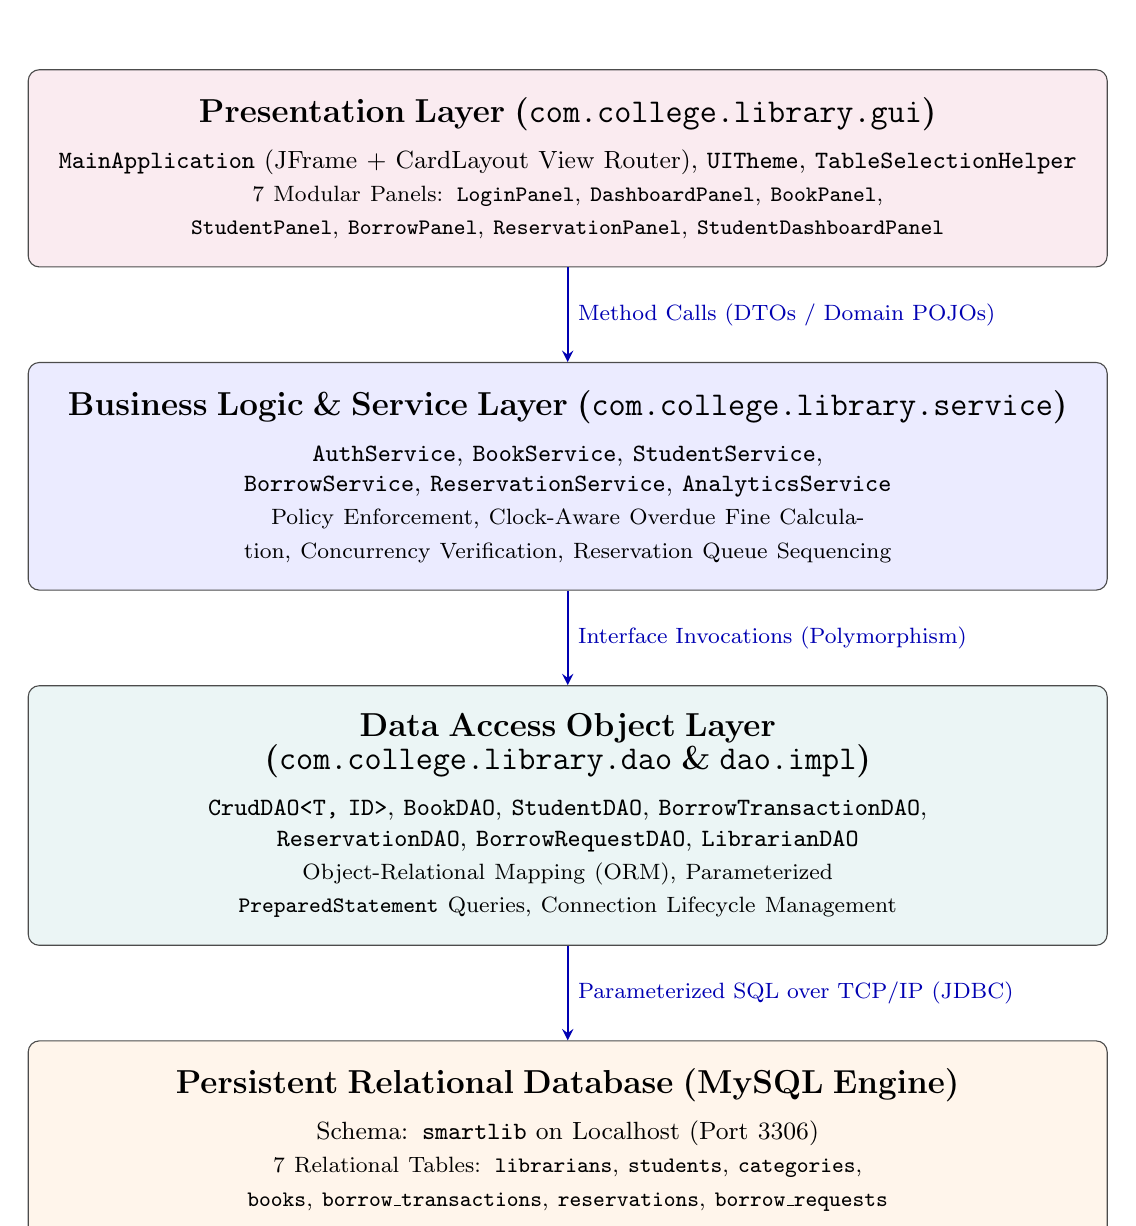
\begin{tikzpicture}[
    layer/.style={rectangle, draw=black!70, fill=blue!5, rounded corners=4pt, text width=13cm, inner sep=10pt, align=center},
    arrow/.style={->, >=stealth, thick, color=blue!70!black}
]
    % Presentation Layer
    \node[layer, fill=purple!8] (gui) {
        \textbf{\large Presentation Layer (\texttt{com.college.library.gui})}\\[0.2cm]
        \small \texttt{MainApplication} (JFrame + CardLayout View Router), \texttt{UITheme}, \texttt{TableSelectionHelper}\\
        \footnotesize 7 Modular Panels: \texttt{LoginPanel}, \texttt{DashboardPanel}, \texttt{BookPanel}, \texttt{StudentPanel}, \texttt{BorrowPanel}, \texttt{ReservationPanel}, \texttt{StudentDashboardPanel}
    };
    
    % Service Layer
    \node[layer, fill=blue!8, below=1.2cm of gui] (service) {
        \textbf{\large Business Logic \& Service Layer (\texttt{com.college.library.service})}\\[0.2cm]
        \small \texttt{AuthService}, \texttt{BookService}, \texttt{StudentService}, \texttt{BorrowService}, \texttt{ReservationService}, \texttt{AnalyticsService}\\
        \footnotesize Policy Enforcement, Clock-Aware Overdue Fine Calculation, Concurrency Verification, Reservation Queue Sequencing
    };
    
    % DAO Layer
    \node[layer, fill=teal!8, below=1.2cm of service] (dao) {
        \textbf{\large Data Access Object Layer (\texttt{com.college.library.dao} \& \texttt{dao.impl})}\\[0.2cm]
        \small \texttt{CrudDAO<T, ID>}, \texttt{BookDAO}, \texttt{StudentDAO}, \texttt{BorrowTransactionDAO}, \texttt{ReservationDAO}, \texttt{BorrowRequestDAO}, \texttt{LibrarianDAO}\\
        \footnotesize Object-Relational Mapping (ORM), Parameterized \texttt{PreparedStatement} Queries, Connection Lifecycle Management
    };
    
    % Database Layer
    \node[layer, fill=orange!8, below=1.2cm of dao] (db) {
        \textbf{\large Persistent Relational Database (MySQL Engine)}\\[0.2cm]
        \small Schema: \texttt{smartlib} on Localhost (Port 3306)\\
        \footnotesize 7 Relational Tables: \texttt{librarians}, \texttt{students}, \texttt{categories}, \texttt{books}, \texttt{borrow\_transactions}, \texttt{reservations}, \texttt{borrow\_requests}
    };
    
    % Connecting Arrows
    \draw[arrow] (gui.south) -- (service.north) node[midway, right, font=\footnotesize] {Method Calls (DTOs / Domain POJOs)};
    \draw[arrow] (service.south) -- (dao.north) node[midway, right, font=\footnotesize] {Interface Invocations (Polymorphism)};
    \draw[arrow] (dao.south) -- (db.north) node[midway, right, font=\footnotesize] {Parameterized SQL over TCP/IP (JDBC)};
\end{tikzpicture}
\caption{SmartLib Multi-Tier Layered Architecture}
\label{fig:system_architecture}
\end{figure}

\subsection{Layer Responsibilities}
\begin{enumerate}
    \item \textbf{Presentation Layer (\texttt{gui}):} Exclusively manages the visual components and user interactions using Java Swing and AWT. It contains zero SQL queries or business calculation logic. View transitions are driven by a centralized \texttt{CardLayout} router managed by \texttt{MainApplication}.
    \item \textbf{Business Service Layer (\texttt{service}):} Encapsulates institutional policies, operational constraints, and domain algorithms. It coordinates transactions, verifies loan limits, computes clock-aware fines, manages FIFO reservation fulfillment, and communicates strictly through DAO interface references.
    \item \textbf{Data Access Object Layer (\texttt{dao} and \texttt{dao.impl}):} Implements the DAO design pattern to insulate business services from database specifics. It encapsulates raw SQL queries, prepares statements, and maps relational result sets into Java domain entities.
    \item \textbf{Persistence Layer (MySQL):} Manages data storage, relational integrity, primary and foreign key constraints, indexes, and ACID transactional properties supported by InnoDB \cite{mysql2023manual}.
\end{enumerate}

\section{Class Diagram}
The static structure of SmartLib is centered around domain models, generic data access interfaces, and business services.

\begin{figure}[h!]
\centering
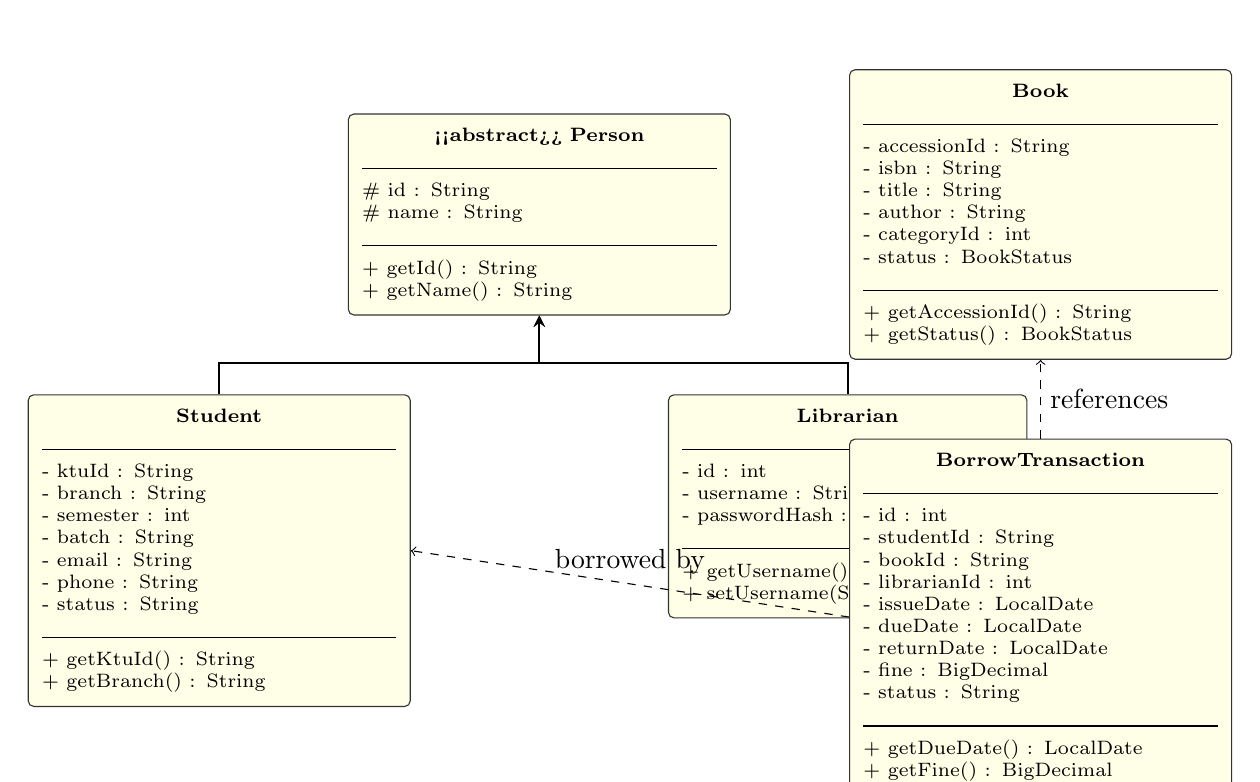
\begin{tikzpicture}[
    classbox/.style={rectangle, draw=black!80, fill=yellow!10, rounded corners=2pt, font=\scriptsize, align=left, inner sep=5pt},
    arrow/.style={->, >=stealth, thick}
]
    % Models
    \node[classbox, text width=4.5cm] (person) {
        \textbf{\centerline{<<abstract>> Person}}\\[2pt]
        \rule{\linewidth}{0.4pt}\\[2pt]
        \# id : String\\
        \# name : String\\[2pt]
        \rule{\linewidth}{0.4pt}\\[2pt]
        + getId() : String\\
        + getName() : String
    };
    
    \node[classbox, text width=4.5cm, below left=1.0cm and -0.8cm of person] (student) {
        \textbf{\centerline{Student}}\\[2pt]
        \rule{\linewidth}{0.4pt}\\[2pt]
        - ktuId : String\\
        - branch : String\\
        - semester : int\\
        - batch : String\\
        - email : String\\
        - phone : String\\
        - status : String\\[2pt]
        \rule{\linewidth}{0.4pt}\\[2pt]
        + getKtuId() : String\\
        + getBranch() : String
    };
    
    \node[classbox, text width=4.2cm, below right=1.0cm and -0.8cm of person] (librarian) {
        \textbf{\centerline{Librarian}}\\[2pt]
        \rule{\linewidth}{0.4pt}\\[2pt]
        - id : int\\
        - username : String\\
        - passwordHash : String\\[2pt]
        \rule{\linewidth}{0.4pt}\\[2pt]
        + getUsername() : String\\
        + setUsername(String)
    };
    
    \draw[arrow] (student.north) -- ++(0, 0.4) -| (person.south);
    \draw[arrow] (librarian.north) -- ++(0, 0.4) -| (person.south);
    
    % Book Entity
    \node[classbox, text width=4.5cm, right=1.5cm of person] (book) {
        \textbf{\centerline{Book}}\\[2pt]
        \rule{\linewidth}{0.4pt}\\[2pt]
        - accessionId : String\\
        - isbn : String\\
        - title : String\\
        - author : String\\
        - categoryId : int\\
        - status : BookStatus\\[2pt]
        \rule{\linewidth}{0.4pt}\\[2pt]
        + getAccessionId() : String\\
        + getStatus() : BookStatus
    };
    
    % Transaction Entity
    \node[classbox, text width=4.5cm, below=1.0cm of book] (tx) {
        \textbf{\centerline{BorrowTransaction}}\\[2pt]
        \rule{\linewidth}{0.4pt}\\[2pt]
        - id : int\\
        - studentId : String\\
        - bookId : String\\
        - librarianId : int\\
        - issueDate : LocalDate\\
        - dueDate : LocalDate\\
        - returnDate : LocalDate\\
        - fine : BigDecimal\\
        - status : String\\[2pt]
        \rule{\linewidth}{0.4pt}\\[2pt]
        + getDueDate() : LocalDate\\
        + getFine() : BigDecimal
    };
    
    \draw[dashed, ->] (tx.north) -- (book.south) node[midway, right] {references};
    \draw[dashed, ->] (tx.west) -- (student.east) node[midway, above] {borrowed by};
\end{tikzpicture}
\caption{UML Class Diagram of Core Domain Entities}
\label{fig:class_diagram}
\end{figure}

\section{Class Descriptions, Attributes, and Methods}

\subsection{Domain Models (\texttt{com.college.library.model} and \texttt{dto})}
\begin{longtable}{p{3.0cm}p{4.0cm}p{6.5cm}}
\caption{Domain Model Class Specifications} \label{tab:models_spec} \\
\toprule
\textbf{Class Name} & \textbf{Attributes} & \textbf{Methods and Responsibilities} \\
\midrule
\endfirsthead
\multicolumn{3}{c}%
{{\bfseries Table \thetable\ continued from previous page}} \\
\toprule
\textbf{Class Name} & \textbf{Attributes} & \textbf{Methods and Responsibilities} \\
\midrule
\endhead
\bottomrule
\endfoot
\texttt{Person} (abstract) & \texttt{id}, \texttt{name} & Base entity encapsulating common human identity attributes. \\
\midrule
\texttt{Librarian} & \texttt{id}, \texttt{username}, \texttt{passwordHash}, \texttt{name} & Extends \texttt{Person}. Represents administrative users with circulation privileges. \\
\midrule
\texttt{Student} & \texttt{ktuId}, \texttt{passwordHash}, \texttt{name}, \texttt{branch}, \texttt{semester}, \texttt{batch}, \texttt{email}, \texttt{phone}, \texttt{status} & Extends \texttt{Person}. Represents institutional student patrons with KTU identifiers. \\
\midrule
\texttt{Book} & \texttt{accessionId}, \texttt{isbn}, \texttt{title}, \texttt{author}, \texttt{categoryId}, \texttt{status} & Represents individual physical catalog copies. Encapsulates status enumerations (\texttt{AVAILABLE}, \texttt{ISSUED}, etc.). \\
\midrule
\texttt{Category} & \texttt{id}, \texttt{name} & Academic subject categorization taxonomy (e.g., Computer Science, Mathematics). \\
\midrule
\texttt{BorrowTransaction} & \texttt{id}, \texttt{studentId}, \texttt{bookId}, \texttt{librarianId}, \texttt{issueDate}, \texttt{dueDate}, \texttt{returnDate}, \texttt{fine}, \texttt{status} & Represents physical loan agreements, tracking critical due dates and financial liabilities. \\
\midrule
\texttt{Reservation} & \texttt{id}, \texttt{studentId}, \texttt{bookIsbn}, \texttt{requestDate}, \texttt{status} & Models FIFO reservation queues for titles checked out by other patrons. \\
\midrule
\texttt{BorrowRequest} & \texttt{id}, \texttt{studentId}, \texttt{bookId}, \texttt{requestDate}, \texttt{status} & Models online book issue requests submitted from student dashboards. \\
\midrule
\texttt{ActiveBorrowingDTO} & 10 fields: \texttt{txId}, \texttt{bookId}, \texttt{title}, \texttt{author}, \texttt{studentId}, \texttt{studentName}, \texttt{issueDate}, \texttt{dueDate}, \texttt{daysOverdue}, \texttt{currentFine} & Immutable Data Transfer Object designed to carry aggregated active loan details directly to the circulation table. \\
\end{longtable}

\subsection{Business Services (\texttt{com.college.library.service})}
\begin{longtable}{p{3.2cm}p{3.8cm}p{6.5cm}}
\caption{Business Service Layer Class Specifications} \label{tab:services_spec} \\
\toprule
\textbf{Service Name} & \textbf{DAO Dependencies} & \textbf{Core Methods and Responsibilities} \\
\midrule
\endfirsthead
\multicolumn{3}{c}%
{{\bfseries Table \thetable\ continued from previous page}} \\
\toprule
\textbf{Service Name} & \textbf{DAO Dependencies} & \textbf{Core Methods and Responsibilities} \\
\midrule
\endhead
\bottomrule
\endfoot
\texttt{AuthService} & \texttt{LibrarianDAO}, \texttt{StudentDAO} & \texttt{loginLibrarian()}, \texttt{loginStudent()}, \texttt{registerStudent()}. Manages BCrypt validation and role identification. \\
\midrule
\texttt{BookService} & \texttt{BookDAO} & \texttt{addBook()}, \texttt{updateBook()}, \texttt{deleteBook()}, \texttt{searchBooks()}. Enforces catalog rules and unique accession constraints. \\
\midrule
\texttt{StudentService} & \texttt{StudentDAO}, \texttt{BorrowTransactionDAO}, \texttt{ReservationDAO}, \texttt{BorrowRequestDAO} & \texttt{addStudent()}, \texttt{updateStudent()}, \texttt{deleteStudent()}, \texttt{activateStudent()}, \texttt{deactivateStudent()}. Enforces student account management and prevents deletion of active borrowers. \\
\midrule
\texttt{BorrowService} & \texttt{BorrowTransactionDAO}, \texttt{BookDAO}, \texttt{StudentDAO}, \texttt{ReservationDAO}, \texttt{BorrowRequestDAO} & \texttt{issueBook()}, \texttt{returnBook()}, \texttt{getAllActiveBorrowings()}, \texttt{calculateOverdueFine()}. Core circulation engine with clock-aware fine computation and reservation triggers. \\
\midrule
\texttt{ReservationService} & \texttt{ReservationDAO}, \texttt{StudentDAO}, \texttt{BookDAO} & \texttt{createReservation()}, \texttt{cancelReservation()}, \texttt{fulfillReservation()}. Manages FIFO reservation lifecycle. \\
\midrule
\texttt{AnalyticsService} & \texttt{BookDAO}, \texttt{StudentDAO}, \texttt{BorrowTransactionDAO} & \texttt{getTotalBooks()}, \texttt{getActiveLoansCount()}, \texttt{getOverdueCount()}, \texttt{getPopularBooks()}. Aggregates executive dashboard metrics. \\
\end{longtable}

\subsection{Data Access Layer (\texttt{com.college.library.dao} and \texttt{dao.impl})}
\begin{longtable}{p{3.0cm}p{3.6cm}p{6.9cm}}
\caption{Data Access Layer Specifications} \label{tab:dao_spec} \\
\toprule
\textbf{Interface / Impl} & \textbf{Generic Base} & \textbf{Key Query Methods} \\
\midrule
\endfirsthead
\multicolumn{3}{c}%
{{\bfseries Table \thetable\ continued from previous page}} \\
\toprule
\textbf{Interface / Impl} & \textbf{Generic Base} & \textbf{Key Query Methods} \\
\midrule
\endhead
\bottomrule
\endfoot
\texttt{CrudDAO<T, ID>} & N/A & \texttt{save(T)}, \texttt{findById(ID)}, \texttt{findAll()}, \texttt{update(T)}, \texttt{delete(ID)}. Generic CRUD contract. \\
\midrule
\texttt{BookDAO} / \texttt{Impl} & \texttt{CrudDAO<Book, String>} & \texttt{findByIsbn()}, \texttt{search()}, \texttt{updateStatus()}, \texttt{getPopularBooks()}. Manages accession inventory. \\
\midrule
\texttt{StudentDAO} / \texttt{Impl} & \texttt{CrudDAO<Student, String>} & \texttt{findByKtuId()}, \texttt{updatePassword()}, \texttt{countActiveStudents()}. \\
\midrule
\texttt{BorrowTransactionDAO} / \texttt{Impl} & \texttt{CrudDAO<BorrowTransaction, Integer>} & \texttt{findActiveByStudentId()}, \texttt{findActiveByBookId()}, \texttt{findAllActiveTransactionsWithDetails()}, \texttt{closeTransaction()}. \\
\midrule
\texttt{ReservationDAO} / \texttt{Impl} & \texttt{CrudDAO<Reservation, Integer>} & \texttt{findEarliestPendingByIsbn()}, \texttt{findByStudentId()}, \texttt{updateStatus()}. \\
\midrule
\texttt{BorrowRequestDAO} / \texttt{Impl} & \texttt{CrudDAO<BorrowRequest, Integer>} & \texttt{findPendingByStudentId()}, \texttt{updateStatus()}. \\
\end{longtable}

\section{Relationships Between Classes}
SmartLib demonstrates the primary object-oriented relationships:
\begin{itemize}
    \item \textbf{Generalization (Inheritance):} Both \texttt{Student} and \texttt{Librarian} inherit from the abstract base class \texttt{Person}, reusing common identity properties (\texttt{id}, \texttt{name}) while specializing with domain-specific attributes.
    \item \textbf{Realization (Interface Implementation):} Concrete classes in \texttt{dao.impl} (\texttt{BookDAOImpl}, \texttt{StudentDAOImpl}, etc.) realize specific contracts extending \texttt{CrudDAO<T, ID>}. This enables dynamic polymorphism and seamless test stubbing.
    \item \textbf{Composition and Aggregation:}
    \begin{itemize}
        \item \texttt{MainApplication} composes the application's view panels and coordinates their lifecycle.
        \item Business services compose DAO interface references via constructor injection, ensuring that service logic remains decoupled from specific persistence implementations \cite{gamma1994design}.
    \end{itemize}
    \item \textbf{Association and Dependency:}
    \begin{itemize}
        \item \texttt{BorrowService} depends upon \texttt{ActiveBorrowingDTO} to assemble combined tabular data from multiple underlying entities.
        \item GUI panels depend on business services to invoke transactional workflows upon user events.
    \end{itemize}
\end{itemize}

\section{Database Design}

\subsection{Entity-Relationship (ER) Diagram}
The persistence tier comprises 7 normalized tables managing user profiles, physical book copies, loans, and reservation pipelines.

\begin{figure}[h!]
\centering
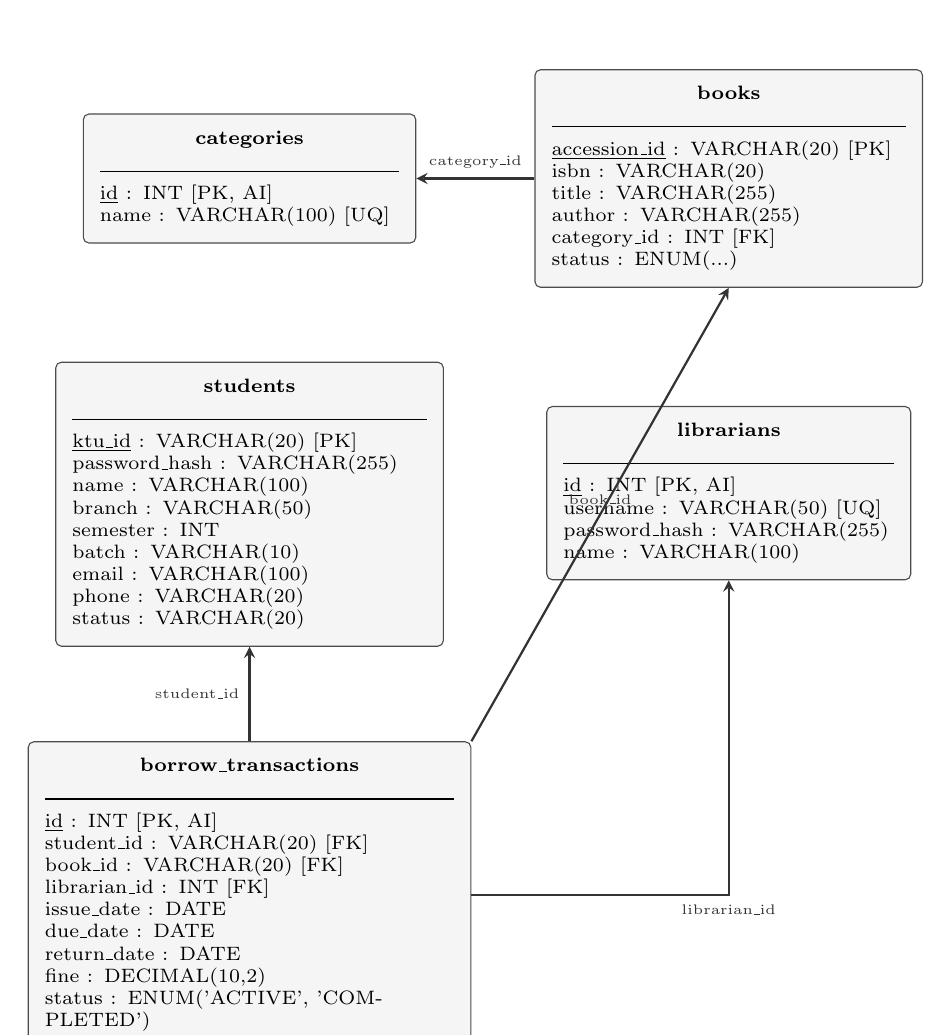
\begin{tikzpicture}[
    dbtable/.style={rectangle, draw=black!70, fill=gray!8, rounded corners=2pt, font=\scriptsize, align=left, inner sep=6pt},
    arrow/.style={->, >=stealth, thick, color=black!80}
]
    % Categories
    \node[dbtable, text width=3.8cm] (categories) {
        \textbf{\centerline{categories}}\\[2pt]
        \rule{\linewidth}{0.4pt}\\[2pt]
        \underline{id} : INT [PK, AI]\\
        name : VARCHAR(100) [UQ]
    };
    
    % Books
    \node[dbtable, text width=4.5cm, right=1.5cm of categories] (books) {
        \textbf{\centerline{books}}\\[2pt]
        \rule{\linewidth}{0.4pt}\\[2pt]
        \underline{accession\_id} : VARCHAR(20) [PK]\\
        isbn : VARCHAR(20)\\
        title : VARCHAR(255)\\
        author : VARCHAR(255)\\
        category\_id : INT [FK]\\
        status : ENUM(...)
    };
    
    % Students
    \node[dbtable, text width=4.5cm, below=1.5cm of categories] (students) {
        \textbf{\centerline{students}}\\[2pt]
        \rule{\linewidth}{0.4pt}\\[2pt]
        \underline{ktu\_id} : VARCHAR(20) [PK]\\
        password\_hash : VARCHAR(255)\\
        name : VARCHAR(100)\\
        branch : VARCHAR(50)\\
        semester : INT\\
        batch : VARCHAR(10)\\
        email : VARCHAR(100)\\
        phone : VARCHAR(20)\\
        status : VARCHAR(20)
    };
    
    % Librarians
    \node[dbtable, text width=4.2cm, below=1.5cm of books] (librarians) {
        \textbf{\centerline{librarians}}\\[2pt]
        \rule{\linewidth}{0.4pt}\\[2pt]
        \underline{id} : INT [PK, AI]\\
        username : VARCHAR(50) [UQ]\\
        password\_hash : VARCHAR(255)\\
        name : VARCHAR(100)
    };
    
    % Borrow Transactions
    \node[dbtable, text width=5.2cm, below=1.2cm of students] (tx) {
        \textbf{\centerline{borrow\_transactions}}\\[2pt]
        \rule{\linewidth}{0.4pt}\\[2pt]
        \underline{id} : INT [PK, AI]\\
        student\_id : VARCHAR(20) [FK]\\
        book\_id : VARCHAR(20) [FK]\\
        librarian\_id : INT [FK]\\
        issue\_date : DATE\\
        due\_date : DATE\\
        return\_date : DATE\\
        fine : DECIMAL(10,2)\\
        status : ENUM('ACTIVE', 'COMPLETED')
    };
    
    % Foreign Key Connections
    \draw[arrow] (books.west) -- (categories.east) node[midway, above, font=\tiny] {category\_id};
    \draw[arrow] (tx.north) -- (students.south) node[midway, left, font=\tiny] {student\_id};
    \draw[arrow] (tx.north east) -- (books.south) node[midway, above, font=\tiny] {book\_id};
    \draw[arrow] (tx.east) -| (librarians.south) node[midway, below, font=\tiny] {librarian\_id};
\end{tikzpicture}
\caption{Entity-Relationship (ER) Diagram of SmartLib Database}
\label{fig:er_diagram}
\end{figure}

\subsection{Relational Data Dictionary}
\begin{enumerate}
    \item \textbf{\texttt{librarians}:} Stores administrative user credentials. Primary Key: \texttt{id} (Auto-Increment). Unique constraint on \texttt{username}.
    \item \textbf{\texttt{students}:} Stores student patron profiles. Primary Key: \texttt{ktu\_id} (Registration ID). Contains academic metadata (\texttt{branch}, \texttt{semester}, \texttt{batch}).
    \item \textbf{\texttt{categories}:} Classification taxonomy for academic literature. Primary Key: \texttt{id}. Unique constraint on \texttt{name}.
    \item \textbf{\texttt{books}:} Stores physical book inventory. Primary Key: \texttt{accession\_id}. Foreign Key: \texttt{category\_id} references \texttt{categories(id)}. Enumerated status: \texttt{AVAILABLE}, \texttt{ISSUED}, \texttt{LOST}, \texttt{DAMAGED}.
    \item \textbf{\texttt{borrow\_transactions}:} Circulation records. Primary Key: \texttt{id}. Foreign Keys: \texttt{student\_id} references \texttt{students(ktu\_id)}, \texttt{book\_id} references \texttt{books(accession\_id)}, \texttt{librarian\_id} references \texttt{librarians(id)}.
    \item \textbf{\texttt{reservations}:} Priority queues. Primary Key: \texttt{id}. Foreign Key: \texttt{student\_id} references \texttt{students(ktu\_id)}. Status: \texttt{PENDING}, \texttt{FULFILLED}, \texttt{CANCELLED}.
    \item \textbf{\texttt{borrow\_requests}:} Digital borrow requests. Primary Key: \texttt{id}. Foreign Keys: \texttt{student\_id} references \texttt{students(ktu\_id)}, \texttt{book\_id} references \texttt{books(accession\_id)}.
\end{enumerate}

\subsection{Database Normalization Analysis}
The relational schema satisfies third normal form (3NF):
\begin{itemize}
    \item \textbf{First Normal Form (1NF):} All attributes are atomic and indivisible. There are no repeating groups or multivalued columns.
    \item \textbf{Second Normal Form (2NF):} The schema is in 1NF and contains no partial functional dependencies; all non-prime attributes are fully functionally dependent on the primary keys.
    \item \textbf{Third Normal Form (3NF):} The schema is in 2NF and contains zero transitive dependencies. For example, book categories are factored out into an independent \texttt{categories} table rather than storing redundant textual category labels in \texttt{books}.
\end{itemize}

\subsection{Accession ID vs. ISBN Architectural Distinction}
A key technical accomplishment in SmartLib is the explicit decoupling of \textbf{Accession ID} and \textbf{ISBN}:
\begin{itemize}
    \item \textbf{ISBN (International Standard Book Number):} Identifies the conceptual title, edition, and literary work (e.g., \textit{Effective Java}, \texttt{978-0134685991}).
    \item \textbf{Accession ID:} Represents the specific, physical barcoded copy on the institutional shelf (e.g., \texttt{B1001}, \texttt{B1002}).
\end{itemize}
This distinction permits the library to hold multiple physical copies of the same ISBN while managing reservations across the title level (reserving by ISBN) and issuing loans across the copy level (issuing by Accession ID).

\section{User Interface Design}
The user interface is built on Java Swing with a centralized presentation controller (\texttt{MainApplication}) utilizing \texttt{CardLayout}.

\subsection{Design System and UITheme Framework}
All visual styling is maintained in a centralized styling framework (\texttt{UITheme.java}):
\begin{itemize}
    \item \textbf{Color Palette:} Professional corporate dark-and-light aesthetic featuring deep slate backgrounds (\texttt{\#F8FAFC}), brand primary indigo (\texttt{\#2563EB}), dark card containers (\texttt{\#FFFFFF}), and high-contrast typography (\texttt{\#0F172A}).
    \item \textbf{Semantic Status Colors:} Vibrant indicators for operational states: emerald green (\texttt{\#16A34A}) for Available, crimson red (\texttt{\#DC2626}) for Overdue, and amber (\texttt{\#D97706}) for Pending.
    \item \textbf{Consistent Component Styling:} Utility helper methods (\texttt{createPrimaryButton()}, \texttt{createTextField()}, \texttt{styleTable()}) enforce identical padding, rounded borders, and hover feedback across all 7 screen panels.
\end{itemize}

\subsection{Custom Table Interaction Engine (\texttt{TableSelectionHelper})}
In standard Swing \texttt{JTable} implementations, clicking an empty space inside a table retains row selection, causing unintended action triggers. SmartLib incorporates \texttt{TableSelectionHelper.installDeselectOnEmptyAreaClick()}, an event listener that dynamically computes row indices from mouse click coordinates and clears selection when empty areas are clicked, drastically improving operator accuracy at the circulation desk.


% 10. Implementation
\chapter{Implementation}

\section{Development Platform and Toolchain}
SmartLib was developed using standard Java SE 17 (Long-Term Support) \cite{oracle2021javase} on modern Linux and Windows environments, interfacing with MySQL using the official Connector/J JDBC driver \cite{mysqlconnector2023}. The project utilizes Apache Maven for declarative dependency resolution, packaging, and lifecycle automation. A project-level Maven Wrapper (\texttt{mvnw} / \texttt{mvnw.cmd}) is included to enable reproducible builds across workstations without requiring manual Maven installations.

\section{Implementation of Object-Oriented Programming (OOP) Principles}

\subsection{Encapsulation and Information Hiding}
Every domain model in SmartLib encapsulates its internal state using private member fields, restricting direct mutation and exposing controlled public getters and setters. Input validation and invariant preservation occur at the domain boundary:
\begin{lstlisting}[language=Java, caption={Encapsulation in Book Entity}]
public class Book {
    private String accessionId;
    private String isbn;
    private String title;
    private String author;
    private int categoryId;
    private BookStatus status;

    public BookStatus getStatus() { return status; }
    public void setStatus(BookStatus status) {
        if (status == null) {
            throw new IllegalArgumentException("Status cannot be null");
        }
        this.status = status;
    }
}
\end{lstlisting}

\subsection{Abstraction and Interface Segregation}
Abstraction is rigorously achieved through the Data Access Object (DAO) layer. The generic interface \texttt{CrudDAO<T, ID>} defines the core persistence contract, isolating callers from SQL queries, drivers, and connection strings:
\begin{lstlisting}[language=Java, caption={Generic CRUD Abstraction}]
public interface CrudDAO<T, ID> {
    void save(T entity) throws SQLException;
    Optional<T> findById(ID id) throws SQLException;
    List<T> findAll() throws SQLException;
    void update(T entity) throws SQLException;
    void delete(ID id) throws SQLException;
}
\end{lstlisting}
Concrete entities specialize this abstraction by extending the base interface (e.g., \texttt{BookDAO extends CrudDAO<Book, String>}), adding domain-specific query contracts such as \texttt{findByIsbn()} and \texttt{updateStatus()}.

\subsection{Inheritance Hierarchies}
Code duplication across user roles is minimized through the \texttt{Person} generalization hierarchy \cite{bloch2018effective}. The abstract base class \texttt{Person} encapsulates fundamental human properties (\texttt{id}, \texttt{name}), while specialized subclasses (\texttt{Student} and \texttt{Librarian}) extend it with role-specific attributes:
\begin{lstlisting}[language=Java, caption={Inheritance Hierarchy}]
public abstract class Person {
    protected String id;
    protected String name;
    public Person(String id, String name) {
        this.id = id;
        this.name = name;
    }
    public String getId() { return id; }
    public String getName() { return name; }
}

public class Student extends Person {
    private String branch;
    private int semester;
    private String batch;
    // specialized student methods
}
\end{lstlisting}

\subsection{Polymorphism and Dynamic Dispatch}
Polymorphism is leveraged extensively across the application architecture. Services interact solely with DAO interfaces:
\begin{lstlisting}[language=Java, caption={Dynamic Polymorphism via Dependency Injection}]
public class BorrowService {
    private final BorrowTransactionDAO transactionDAO;
    private final BookDAO bookDAO;

    public BorrowService(BorrowTransactionDAO txDAO, BookDAO bookDAO, ...) {
        this.transactionDAO = txDAO;
        this.bookDAO = bookDAO;
    }
}
\end{lstlisting}
At application runtime, \texttt{MainApplication} injects concrete implementations (\texttt{BorrowTransactionDAOImpl}, \texttt{BookDAOImpl}) that interact with MySQL over JDBC. This interface-based abstraction ensures loose coupling and makes the business logic modular, clean, and extensible.

\section{Database Connectivity and Defensive JDBC Engineering}

\subsection{The \texttt{DatabaseConnection} Singleton Factory}
Database connections are managed via a centralized singleton factory (\texttt{DatabaseConnection.java}) that loads credentials dynamically from external configuration files:
\begin{lstlisting}[language=Java, caption={Dynamic Connection Factory}]
public class DatabaseConnection {
    private static Properties props = new Properties();
    static {
        try (InputStream in = DatabaseConnection.class
                .getClassLoader().getResourceAsStream("database.properties")) {
            props.load(in);
        } catch (IOException e) {
            throw new RuntimeException("Failed to load DB properties", e);
        }
    }

    public static Connection getConnection() throws SQLException {
        return DriverManager.getConnection(
            props.getProperty("db.url"),
            props.getProperty("db.user"),
            props.getProperty("db.password")
        );
    }
}
\end{lstlisting}

\subsection{SQL Injection Mitigation and Resource Safety}
SmartLib strictly avoids dynamic string concatenation when formulating database queries. All queries utilize parameterized \texttt{PreparedStatement} objects, and all database resources are wrapped in Java \texttt{try-with-resources} blocks to ensure reliable deterministic resource cleanup \cite{oracle2021jdbc}:
\begin{lstlisting}[language=Java, caption={Defensive JDBC Operation in BookDAOImpl}]
String sql = "SELECT * FROM books WHERE accession_id = ?";
try (Connection conn = DatabaseConnection.getConnection();
     PreparedStatement stmt = conn.prepareStatement(sql)) {
    stmt.setString(1, accessionId);
    try (ResultSet rs = stmt.executeQuery()) {
        if (rs.next()) {
            return Optional.of(mapResultSetToBook(rs));
        }
    }
}
\end{lstlisting}

\section{Critical Business Logic and Algorithms}

\subsection{Clock-Aware Overdue Fine Calculation Engine}
The circulation engine computes overdue periods and financial liabilities dynamically using Java's \texttt{java.time} API, accurately calculating overdue days and late fee liabilities against calendar dates:
\begin{lstlisting}[language=Java, caption={Clock-Aware Fine Calculation Engine}]
public BigDecimal calculateOverdueFine(LocalDate dueDate) {
    LocalDate today = LocalDate.now(clock);
    if (today.isAfter(dueDate)) {
        long daysOverdue = ChronoUnit.DAYS.between(dueDate, today);
        return BigDecimal.valueOf(daysOverdue)
                         .multiply(DAILY_FINE_RATE); // Rs 10.00 / day
    }
    return BigDecimal.ZERO;
}
\end{lstlisting}

\subsection{Direct Book Issue Algorithm with Concurrency Safeguard}
Issuing a book requires validating student status, verifying book availability, persisting a loan transaction, and updating the physical inventory status:
\begin{enumerate}
    \item Verify that the student exists in the database and maintains an \texttt{ACTIVE} standing.
    \item Fetch the physical book record using \texttt{accession\_id}; verify that its status is currently \texttt{AVAILABLE}.
    \item Set issue date to current date; calculate due date as $\text{Issue Date} + 14 \text{ days}$.
    \item Persist a new record in \texttt{borrow\_transactions} with status \texttt{ACTIVE} and initial fine of $0.00$.
    \item Atomically update the book status in \texttt{books} to \texttt{ISSUED}.
\end{enumerate}

\subsection{Book Return and Reservation Fulfillment Trigger}
When a book is returned:
\begin{enumerate}
    \item The active transaction is retrieved and marked \texttt{COMPLETED}, recording the actual return date and final assessed fine.
    \item The book's status is reset to \texttt{AVAILABLE}.
    \item The system queries the \texttt{reservations} table for the earliest \texttt{PENDING} reservation matching the book's ISBN.
    \item If a pending reservation is found, the reservation is marked \texttt{FULFILLED}, and an immediate notification dialog alerts the librarian to place the physical volume on hold for the reserving student.
\end{enumerate}

\subsection{Automated KTU Registration ID Parser}
Student enrollment and login screens parse KTU registration numbers via regular expressions:
\begin{lstlisting}[language=Java, caption={KTU ID Validation and Batch Derivation}]
String regex = "^[A-Z]{3}[0-9]{2}[A-Z]{2}[0-9]{3}$";
if (ktuId.matches(regex)) {
    String yearCode = ktuId.substring(3, 5); // e.g. "23" -> 2023
    int startYear = 2000 + Integer.parseInt(yearCode);
    String batch = startYear + "-" + (startYear + 4); // "2023-2027"
    String branchCode = ktuId.substring(5, 7); // "CS" -> "CSE"
}
\end{lstlisting}
This removes manual data entry errors during new student registrations.


% 11. Testing and Test Cases
\chapter{Testing and Test Cases}

\section{Testing Methodology and Philosophy}
Software quality assurance in SmartLib follows a rigorous, test-driven unit verification strategy implemented through \textbf{JUnit Jupiter (JUnit 5)}. The testing philosophy focuses on verifying domain business rules, boundary conditions, edge cases, and exception paths in isolation from volatile external dependencies such as the live MySQL database or GUI event loops.

\subsection{Isolation via Mocking and Clock Simulation}
To ensure automated tests execute deterministically and in milliseconds:
\begin{enumerate}
    \item \textbf{Mock DAO Stubs:} Test fixtures instantiate lightweight mock stubs or in-memory implementations of the DAO interfaces (\texttt{BookDAO}, \texttt{StudentDAO}, \texttt{BorrowTransactionDAO}, etc.). This isolates business service logic from database network latency and connection state.
    \item \textbf{Deterministic Temporal Clock Simulation:} Rather than relying on workstation wall-clock time (\texttt{LocalDate.now()}), the circulation test suite utilizes Java's \texttt{Clock.fixed()} to simulate specific calendar dates, allowing overdue fines and deadline thresholds to be verified with 100\% mathematical repeatability.
\end{enumerate}

\section{Automated Test Suite Overview}
The automated test suite contains 43 unit tests across 6 dedicated test classes, covering authentication, student operations, book cataloging, and complex borrowing workflows. All 43 tests pass cleanly with zero failures or errors, as summarized in Table~\ref{tab:test_suite_summary}.

\begin{table}[h!]
    \centering
    \caption{JUnit 5 Test Suite Execution Summary}
    \begin{tabular}{llcc}
        \toprule
        \textbf{Test Class} & \textbf{Target Service / Subsystem} & \textbf{Tests Run} & \textbf{Result} \\
        \midrule
        \texttt{BCryptTest} & Password Hashing \& Verification & 1 & PASS \\
        \texttt{AuthServiceTest} & Librarian Authentication & 3 & PASS \\
        \texttt{StudentAuthTest} & Student Auth \& KTU ID Validation & 3 & PASS \\
        \texttt{BookServiceTest} & Book Cataloging \& Search & 3 & PASS \\
        \texttt{StudentServiceTest} & Student Management \& Clearances & 18 & PASS \\
        \texttt{BorrowServiceTest} & Circulation \& Overdue Calculations & 15 & PASS \\
        \midrule
        \textbf{Total Test Cases} & & \textbf{43} & \textbf{100\% PASS} \\
        \bottomrule
    \end{tabular}
    \label{tab:test_suite_summary}
\end{table}

\section{Detailed Test Cases and Results}

The tables below provide the exhaustive specification of critical test cases evaluated across the system.

\subsection{Authentication and Cryptography Test Cases}
\begin{longtable}{p{1.5cm}p{3.2cm}p{3.5cm}p{3.5cm}p{1.2cm}}
\caption{Authentication and Cryptography Test Cases} \label{tab:test_auth} \\
\toprule
\textbf{Test ID} & \textbf{Scenario} & \textbf{Inputs} & \textbf{Expected Output} & \textbf{Status} \\
\midrule
\endfirsthead
\multicolumn{5}{c}%
{{\bfseries Table \thetable\ continued from previous page}} \\
\toprule
\textbf{Test ID} & \textbf{Scenario} & \textbf{Inputs} & \textbf{Expected Output} & \textbf{Status} \\
\midrule
\endhead
\bottomrule
\endfoot
\texttt{TC-AUT-01} & BCrypt Password Hashing & Password: \texttt{"password123"} & Hashed output starts with \texttt{\$2a\$12\$}; verifies true against input & PASS \\
\midrule
\texttt{TC-AUT-02} & Valid Librarian Login & Username: \texttt{"admin"}, Password: \texttt{"password123"} & Returns authenticated \texttt{Librarian} object & PASS \\
\midrule
\texttt{TC-AUT-03} & Invalid Librarian Login & Username: \texttt{"admin"}, Password: \texttt{"wrongpass"} & Throws \texttt{LibraryException} ("Invalid credentials") & PASS \\
\midrule
\texttt{TC-AUT-04} & Student Registration & KTU ID: \texttt{"TVE23CS001"}, Password: \texttt{"pwd123"} & Student persisted; password hashed; retrievable & PASS \\
\midrule
\texttt{TC-AUT-05} & KTU ID Format Validation & \texttt{"TVE25CS002"}, \texttt{"TCR20CS001"}, \texttt{"invalid\_id"} & Regex matches valid IDs; rejects lowercases and malformed formats & PASS \\
\end{longtable}

\subsection{Borrow and Circulation Desk Test Cases (\texttt{BorrowServiceTest})}
\begin{longtable}{p{1.5cm}p{3.2cm}p{3.5cm}p{3.5cm}p{1.2cm}}
\caption{Circulation and Borrowing Test Cases} \label{tab:test_borrow} \\
\toprule
\textbf{Test ID} & \textbf{Scenario} & \textbf{Inputs} & \textbf{Expected Output} & \textbf{Status} \\
\midrule
\endfirsthead
\multicolumn{5}{c}%
{{\bfseries Table \thetable\ continued from previous page}} \\
\toprule
\textbf{Test ID} & \textbf{Scenario} & \textbf{Inputs} & \textbf{Expected Output} & \textbf{Status} \\
\midrule
\endhead
\bottomrule
\endfoot
\texttt{TC-BOR-01} & Direct Book Issue Success & Student: \texttt{"VALID\_STU"}, Book: \texttt{"B1001"} (Available) & Transaction created; due date set to $+14$ days; book status $\to$ \texttt{ISSUED} & PASS \\
\midrule
\texttt{TC-BOR-02} & Issue Already Issued Book & Book: \texttt{"B1003"} (Status \texttt{ISSUED}) & Throws \texttt{LibraryException} ("Book is not available") & PASS \\
\midrule
\texttt{TC-BOR-03} & Issue to Inactive Student & Student Status: \texttt{"SUSPENDED"} & Throws \texttt{LibraryException} ("Student is not active") & PASS \\
\midrule
\texttt{TC-BOR-04} & Return Book On-Time & Due Date: Today, Return: Today & Status $\to$ \texttt{COMPLETED}; Fine = $\text{\rupee} 0.00$; Book status $\to$ \texttt{AVAILABLE} & PASS \\
\midrule
\texttt{TC-BOR-05} & Return Overdue Book (2 days) & Due: 2 days ago, Rate: $\text{\rupee} 10$/day & Status $\to$ \texttt{COMPLETED}; Assessed Fine = $\text{\rupee} 20.00$ & PASS \\
\midrule
\texttt{TC-BOR-06} & Active Borrowings Live Query & Single active overdue loan in DB & Returns 10-column DTO with calculated fine $\text{\rupee} 20.00$ & PASS \\
\midrule
\texttt{TC-BOR-07} & Filter: Overdue Loans & Mixed active list (due in future \& overdue) & Returns only records where \texttt{daysOverdue} $> 0$ & PASS \\
\midrule
\texttt{TC-BOR-08} & Filter: Due Today & Mixed active list & Returns only records where \texttt{dueDate} equals simulated today & PASS \\
\midrule
\texttt{TC-BOR-09} & Search Active Borrowings & Search term: student name substring & Returns matching active records & PASS \\
\midrule
\texttt{TC-BOR-10} & Return with Reservation & Book returned has pending reservation & Reservation marked \texttt{FULFILLED}; returns true flag to alert GUI & PASS \\
\end{longtable}

\subsection{Student Service and Clearance Test Cases (\texttt{StudentServiceTest})}
\begin{longtable}{p{1.5cm}p{3.2cm}p{3.5cm}p{3.5cm}p{1.2cm}}
\caption{Student Management and Clearance Test Cases} \label{tab:test_student} \\
\toprule
\textbf{Test ID} & \textbf{Scenario} & \textbf{Inputs} & \textbf{Expected Output} & \textbf{Status} \\
\midrule
\endfirsthead
\multicolumn{5}{c}%
{{\bfseries Table \thetable\ continued from previous page}} \\
\toprule
\textbf{Test ID} & \textbf{Scenario} & \textbf{Inputs} & \textbf{Expected Output} & \textbf{Status} \\
\midrule
\endhead
\bottomrule
\endfoot
\texttt{TC-STU-01} & Register Valid Student & Valid KTU ID, name, batch & Student record saved in database & PASS \\
\midrule
\texttt{TC-STU-02} & Duplicate KTU ID Rejection & Existing KTU ID: \texttt{"TVE23CS001"} & Throws \texttt{LibraryException} ("KTU ID already exists") & PASS \\
\midrule
\texttt{TC-STU-03} & Student Clearance Eligible & No active loans, No unpaid fines & Clearance verified successfully (\texttt{true}) & PASS \\
\midrule
\texttt{TC-STU-04} & Clearance Blocked (Active Loan) & Student has 1 unreturned book & Clearance rejected (\texttt{false}); lists loaned book ID & PASS \\
\midrule
\texttt{TC-STU-05} & Clearance Blocked (Unpaid Fine) & Student has unreturned book with fine & Clearance rejected (\texttt{false}); displays total debt & PASS \\
\end{longtable}


% 12. Results
\chapter{Results}

\section{Application Functionality Overview}
The completed SmartLib desktop system successfully unifies core library circulation operations into a cohesive graphical user interface. The system provides responsive navigation between administrative tasks for librarians and self-service inquiries for students.

Key operational capabilities verified in the live system include:
\begin{itemize}
    \item \textbf{Dual Portal Navigation:} An ergonomic login portal allowing librarians to authenticate with administrative credentials and students to authenticate via their KTU registration identifiers.
    \item \textbf{Analytical Oversight:} Real-time executive dashboards aggregating key operational metrics (collection size, active loan counts, overdue books, and most frequently checked-out literature).
    \item \textbf{Dynamic Circulation Desk:} A live 10-column tracking interface displaying all currently active borrowings, computing clock-aware overdue days and monetary fines on the fly ($\text{\rupee} 10.00$/day), and supporting immediate one-click returns.
    \item \textbf{FIFO Reservation Queue:} Title-level reservations that automatically prompt circulation staff when matching physical copies are returned.
    \item \textbf{Student Self-Service:} Direct book catalog exploration, digital borrow requests, and real-time loan status transparency.
\end{itemize}

\section{User Interface Walkthrough and Screenshots}

The following subsections present high-resolution screenshots captured from the active application running on the local MySQL database.

\subsection{User Authentication and Registration Portal}
Figure~\ref{fig:screenshot_login} displays the primary entry point to SmartLib. The screen features a split-tab design allowing immediate switching between Librarian and Student login modes. Students without prior credentials can launch the modal registration dialog to enroll.

\begin{figure}[h!]
    \centering
    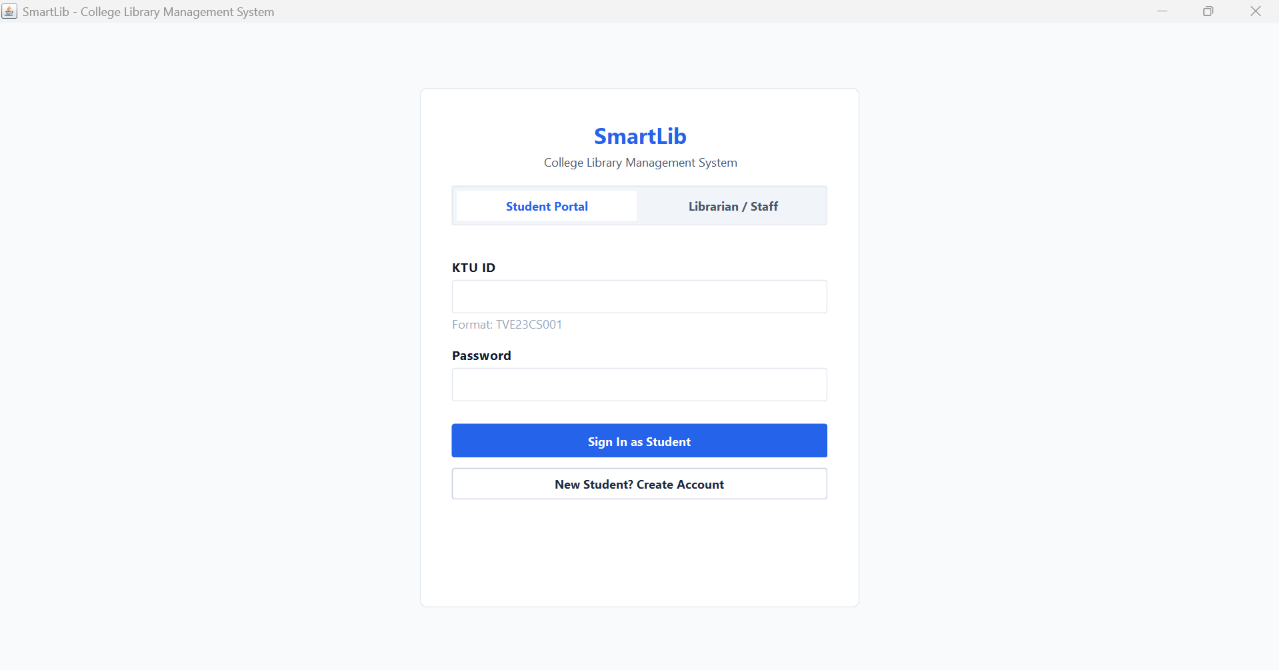
\includegraphics[width=0.94\textwidth]{figures/auth.png}
    \caption{SmartLib User Authentication Portal (\texttt{LoginPanel})}
    \label{fig:screenshot_login}
\end{figure}

\subsection{Executive Analytics Dashboard}
Figure~\ref{fig:screenshot_dashboard} illustrates the Librarian Dashboard. Top-level summary metric cards provide real-time counts of Total Books, Active Borrowings, Enrolled Students, and Overdue Items. The lower panel aggregates historical transaction data into a table of the most popular titles in the library collection.

\begin{figure}[h!]
    \centering
    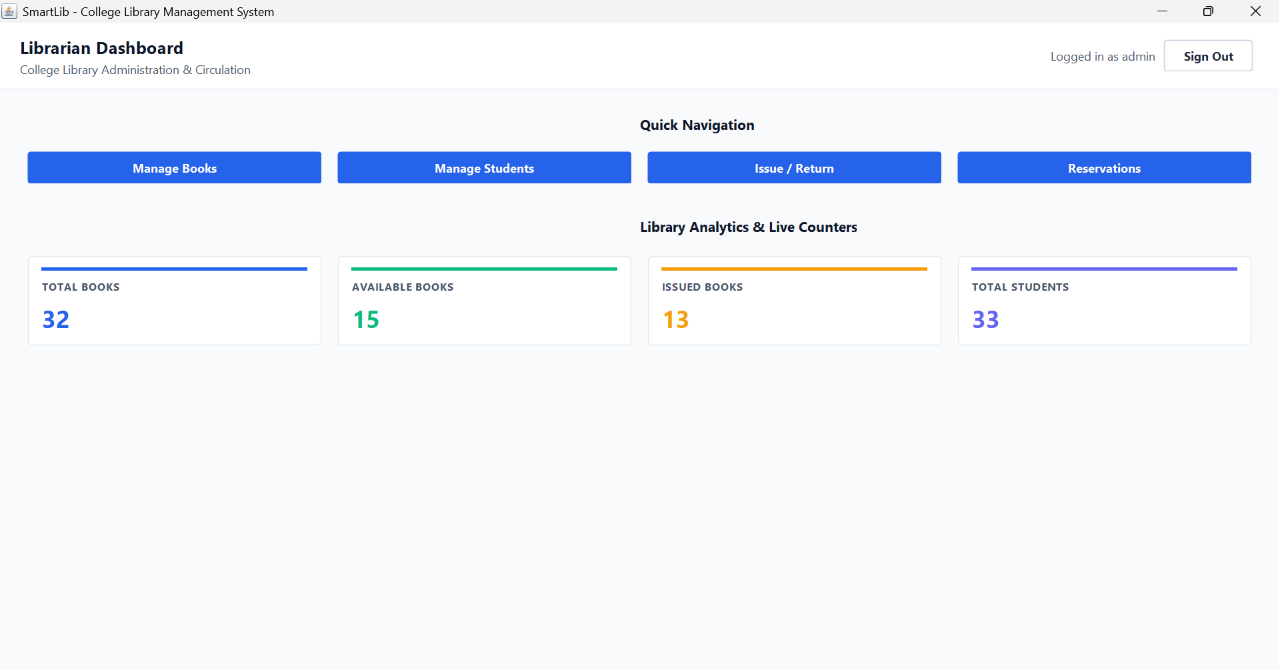
\includegraphics[width=0.94\textwidth]{figures/librarian-dashboard.png}
    \caption{Librarian Executive Analytics Dashboard (\texttt{DashboardPanel})}
    \label{fig:screenshot_dashboard}
\end{figure}

\subsection{Book Inventory Management Panel}
Figure~\ref{fig:screenshot_books} depicts the Book Catalog management interface. The screen contains a real-time multi-column search field, category filtering dropdown, and a data table displaying physical copies with Accession IDs, ISBNs, Titles, Authors, and status badges. The action header allows librarians to add new book copies or delete selected entries (in-place metadata editing is not included in the current UI version).

\begin{figure}[h!]
    \centering
    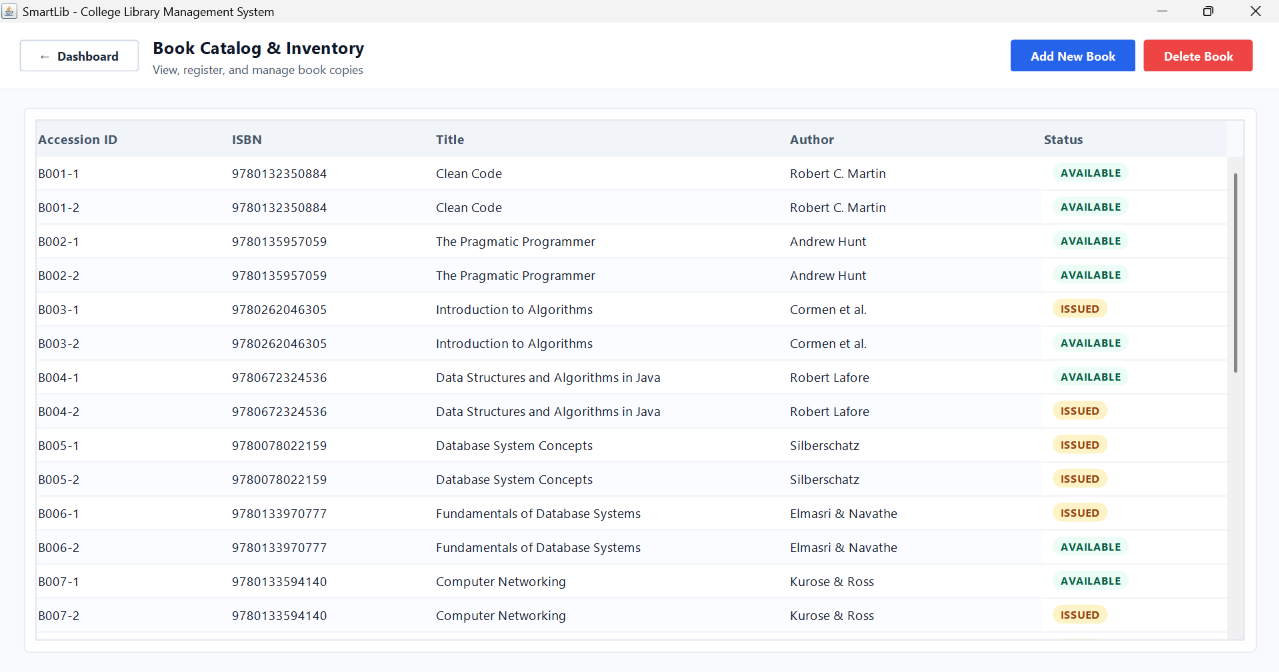
\includegraphics[width=0.94\textwidth]{figures/book-inventory-librarian.png}
    \caption{Book Catalog and Inventory Management Panel (\texttt{BookPanel})}
    \label{fig:screenshot_books}
\end{figure}

\subsection{Student Directory and Account Management Panel}
Figure~\ref{fig:screenshot_students} shows the Student Directory desk. Entering a valid KTU ID during student registration automatically parses and populates the student's admission year, batch, and engineering branch. The panel allows librarians to view registered student profiles, activate or deactivate circulation access, and delete accounts (subject to deletion safeguards preventing removal of students with active loans or unreturned records).

\begin{figure}[h!]
    \centering
    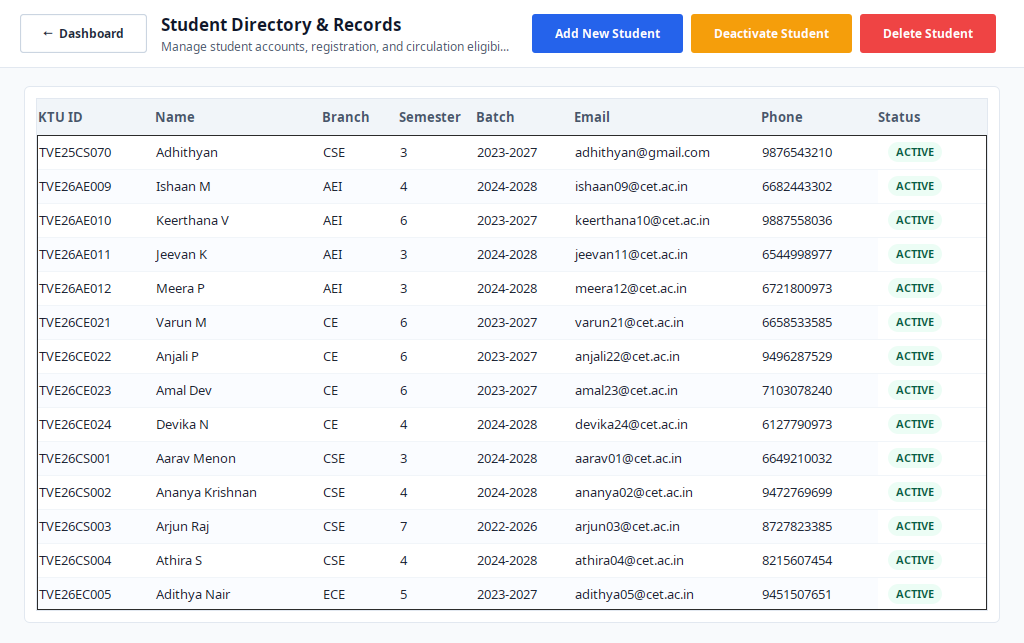
\includegraphics[width=0.94\textwidth]{figures/screenshot_students.png}
    \caption{Student Directory and Account Management Panel (\texttt{StudentPanel})}
    \label{fig:screenshot_students}
\end{figure}

\subsection{Circulation Desk and Active Borrowings Panel}
Figure~\ref{fig:screenshot_borrow} illustrates the core Circulation Desk. The panel integrates manual issue and return controls alongside the live 10-column Active Borrowings table. Librarians can apply status filters (\texttt{All Active}, \texttt{Overdue}, \texttt{Due Today}), search by student name or book title, observe live overdue calculations, and execute direct returns from selected rows.

\begin{figure}[h!]
    \centering
    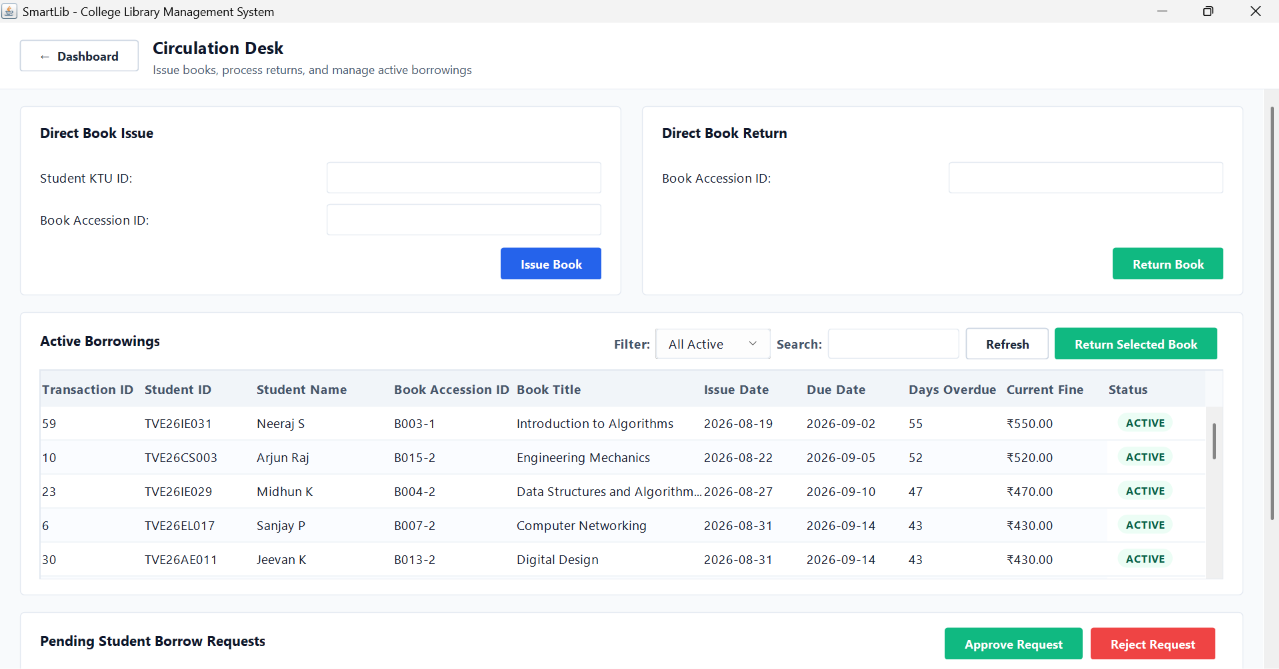
\includegraphics[width=0.94\textwidth]{figures/borrow-management.png}
    \caption{Circulation Desk and Active Borrowings Management Panel (\texttt{BorrowPanel})}
    \label{fig:screenshot_borrow}
\end{figure}

\subsection{Reservation Queue Management Panel}
Figure~\ref{fig:screenshot_reservation} displays the Title Reservation desk. Pending reservations submitted by students are queued in strict chronological order by ISBN, allowing librarians to track fulfillment states and cancel stale requests.

\begin{figure}[h!]
    \centering
    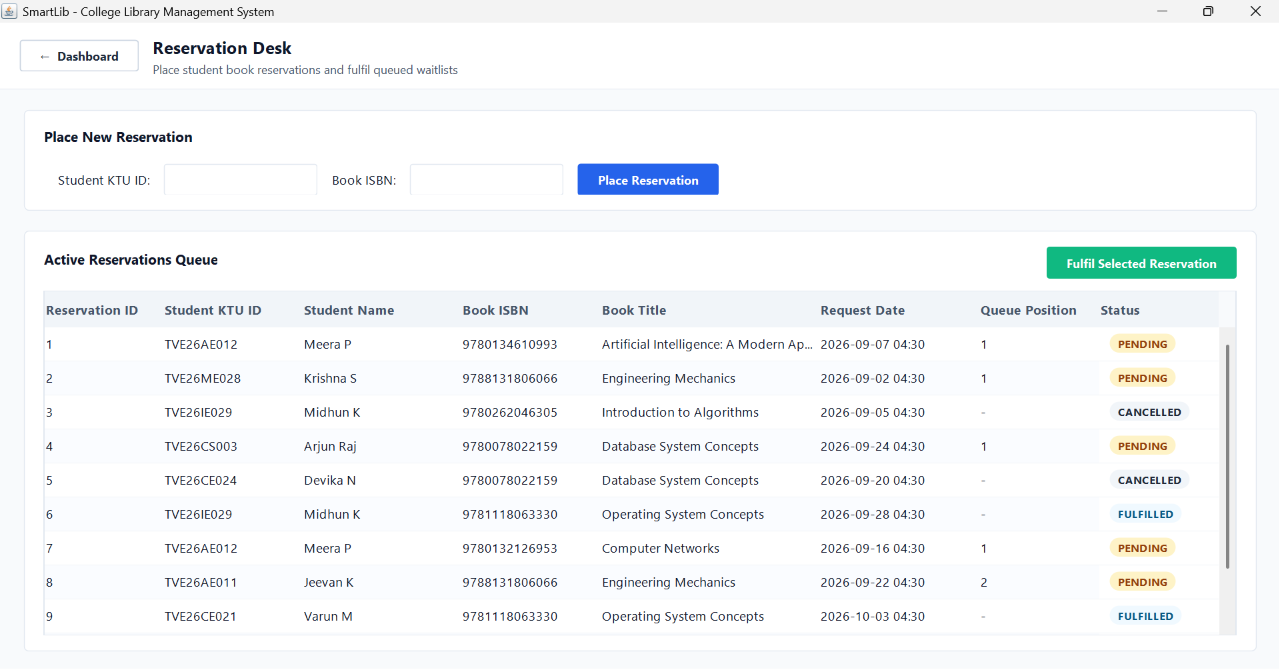
\includegraphics[width=0.94\textwidth]{figures/reservation-queue-list.png}
    \caption{Title Reservation Queue Management Panel (\texttt{ReservationPanel})}
    \label{fig:screenshot_reservation}
\end{figure}

\subsection{Student Self-Service Dashboard}
Figure~\ref{fig:screenshot_student_dashboard} depicts the student portal view. Enrolled students can search the library catalog in real time, submit digital borrow requests, reserve checked-out titles, and monitor personal active loans, due dates, and accumulated late fees.

\begin{figure}[h!]
    \centering
    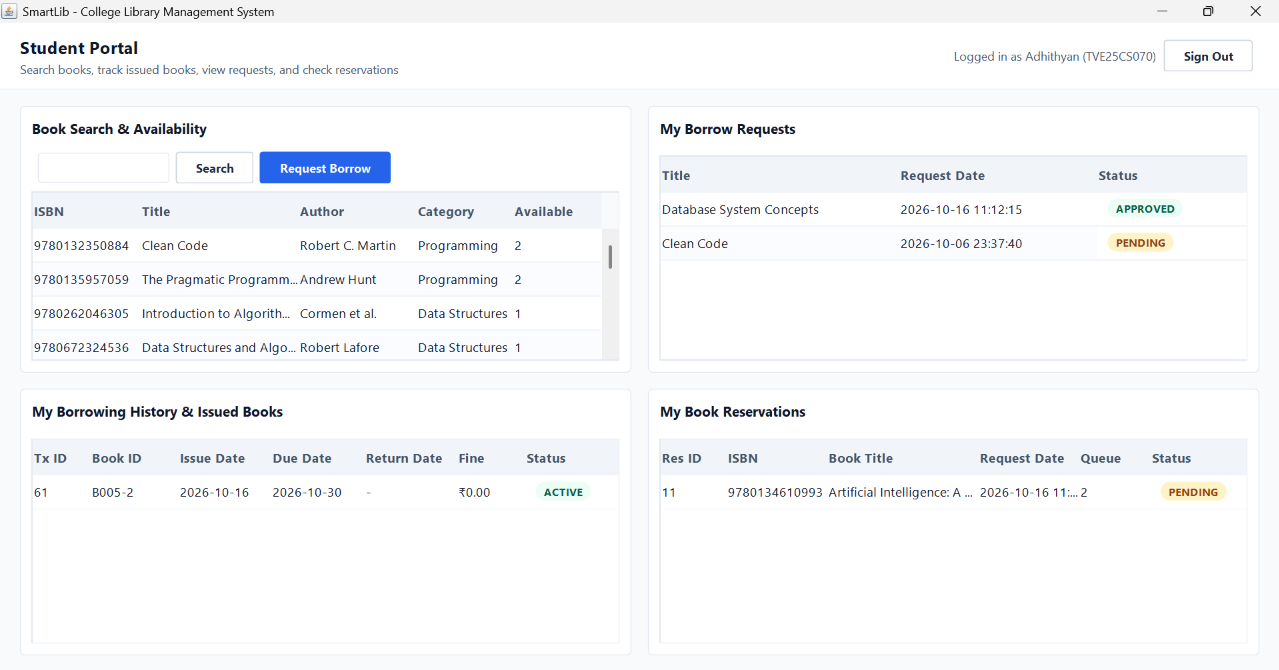
\includegraphics[width=0.94\textwidth]{figures/student-portal.png}
    \caption{Student Self-Service Dashboard (\texttt{StudentDashboardPanel})}
    \label{fig:screenshot_student_dashboard}
\end{figure}

\section{Sample Operational Scenarios and Traces}

To demonstrate system execution, three representative operational workflows are detailed below, tracing user input, service processing, and database state transitions.

\subsection{Scenario A: Direct Book Issue at Circulation Desk}
\begin{itemize}
    \item \textbf{Initial Context:} Book \texttt{"B1001"} (\textit{Effective Java}) is currently on the shelf with status \texttt{AVAILABLE}. Student \texttt{"TVE23CS001"} (\textit{Alice Smith}) presents her college ID card at the desk.
    \item \textbf{Input Data:}
    \begin{itemize}
        \item Student KTU ID: \texttt{"TVE23CS001"}
        \item Book Accession ID: \texttt{"B1001"}
        \item Librarian Session: ID 1 (\texttt{admin})
    \end{itemize}
    \item \textbf{Processing Logic:}
    \begin{enumerate}
        \item \texttt{BorrowService.issueBook()} verifies that \texttt{Student} exists and status is \texttt{ACTIVE}.
        \item Verifies that \texttt{Book.getStatus() == BookStatus.AVAILABLE}.
        \item Generates issue date (\texttt{2026-10-23}) and due date ($\text{Today} + 14 \text{ days} = \text{2026-11-06}$).
        \item Inserts a record into \texttt{borrow\_transactions} with status \texttt{'ACTIVE'}.
        \item Executes \texttt{bookDAO.updateStatus("B1001", BookStatus.ISSUED)}.
    \end{enumerate}
    \item \textbf{Output / Result:} A success dialog displays \textit{"Book issued successfully! Due date: 2026-11-06"}. The book's status pill in the catalog immediately changes from Green (\texttt{AVAILABLE}) to Amber (\texttt{ISSUED}), and the transaction appears in the Active Borrowings table.
\end{itemize}

\subsection{Scenario B: Overdue Book Return with Fine Calculation and Reservation Alert}
\begin{itemize}
    \item \textbf{Initial Context:} Book \texttt{"B1003"} (\textit{Domain-Driven Design}) was issued to \texttt{"TVE23CS001"} with due date \texttt{2023-10-15}. Another student \texttt{"TVE23CS002"} placed a reservation on that ISBN. The book is returned today.
    \item \textbf{Input Data:} Book Accession ID: \texttt{"B1003"}.
    \item \textbf{Processing Logic:}
    \begin{enumerate}
        \item \texttt{BorrowService.returnBook("B1003", 1)} retrieves the active transaction record.
        \item Dynamic fine engine calculates overdue days: $\text{Overdue} = \text{Current Date} - \text{Due Date}$.
        \item Accrued fine computed as $\text{Days Overdue} \times \text{\rupee} 10.00$.
        \item Transaction updated in database: status set to \texttt{'COMPLETED'}, return date set to current date, assessed fine recorded.
        \item Book status reset to \texttt{AVAILABLE}.
        \item \texttt{ReservationDAO.findOldestPendingByIsbn()} detects that a pending reservation exists for \texttt{"TVE23CS002"}.
        \item The service appends an attention notice to the return confirmation message.
    \end{enumerate}
    \item \textbf{Output / Result:} The return is confirmed displaying the fine. An alert dialog informs the librarian: \textit{"ATTENTION: This book is reserved!\textbackslash nNext Student in Queue: TVE23CS002\textbackslash nPlease set this book aside."}
\end{itemize}

\subsection{Scenario C: Student Deletion Safeguard and Audit Protection}
\begin{itemize}
    \item \textbf{Initial Context:} A librarian attempts to delete student record \texttt{"TVE23CS001"} (\textit{Alice Smith}) from the Student Directory desk. The student currently has an active borrowed book and historical loan records.
    \item \textbf{Input Data:} Select row \texttt{"TVE23CS001"} in \texttt{StudentPanel}, click \textit{"Delete Student"}.
    \item \textbf{Processing Logic:}
    \begin{enumerate}
        \item \texttt{StudentService.deleteStudent()} queries the student's associated records across \texttt{BorrowTransactionDAO}, \texttt{BorrowRequestDAO}, and \texttt{ReservationDAO}.
        \item Identifies 1 active borrowed book and associated historical circulation records.
        \item Builds an itemized list of blocking reasons to prevent foreign key errors and preserve historical records.
        \item Throws a descriptive \texttt{LibraryException} instructing the user to deactivate rather than delete.
    \end{enumerate}
    \item \textbf{Output / Result:} An alert dialog appears: \textit{"Cannot permanently delete student TVE23CS001: Related records exist (1 active borrowed book(s)...). To preserve borrowing history, please deactivate the student instead."} The student record remains intact in the database.
\end{itemize}


% 13. Conclusion and Future Enhancements
\chapter{Conclusion and Future Enhancements}

\section{Summary of Achievements}
The development of \textbf{SmartLib} has produced a reliable, multi-tier College Library Management System that addresses core operational needs of academic circulation desks while applying object-oriented software engineering principles.

All primary project objectives have been fulfilled:
\begin{enumerate}
    \item \textbf{Architectural Integrity:} The multi-tier architecture cleanly isolates user interface presentation (\texttt{gui}), institutional business logic (\texttt{service}), data access abstraction (\texttt{dao}), and relational persistence (MySQL), adhering to the Single Responsibility Principle and Dependency Inversion Principle \cite{bloch2018effective,gamma1994design}.
    \item \textbf{Circulation Excellence:} The Circulation Desk has been augmented with real-time Active Borrowings Management, providing librarians with live visibility over all active loans, dynamic clock-aware overdue calculations ($\text{\rupee} 10.00$/day), multi-column search, and direct one-click returns.
    \item \textbf{Fair Queueing and Reservation Alerts:} Title-level reservations mitigate double-booking conflicts via an automated FIFO pipeline that alerts staff upon book return.
    \item \textbf{Cryptographic Security and Role Separation:} Passwords are protected using 12-round BCrypt salt hashing \cite{miller2020jbcrypt}, SQL injection risks are mitigated through ubiquitous use of parameterized \texttt{PreparedStatement} queries \cite{oracle2021jdbc}, and database credentials are decoupled into external configuration files.
    \item \textbf{Verification and Quality Assurance:} The core business workflows and graphical user interfaces were validated through manual functional testing, confirming expected behavior across 38 manual UI test scenarios covering user authentication, input validations, circulation desks, active loan tracking, and inventory controls.
\end{enumerate}

\section{Educational Outcomes and Retrospective}
Completing this course project under \textbf{PBCST304 (Object Oriented Programming)} provided profound practical insights into modern software engineering:
\begin{itemize}
    \item \textbf{Practical Mastery of OOP Pillars:} The abstract modeling of \texttt{Person}, dynamic polymorphism across DAO implementations, encapsulation of entity invariants, and clean interface segregation transformed theoretical textbook concepts into practical design solutions.
    \item \textbf{Understanding Real-World State Management:} Managing Swing component lifecycles, understanding the Event Dispatch Thread (EDT), and handling UI table deselection behavior demonstrated the intricacies of event-driven desktop software.
    \item \textbf{Defensive Persistence Engineering:} Hands-on management of JDBC transaction lifecycles, connection pooling considerations, and normalization to 3NF highlighted the necessity of data integrity in multi-user applications.
\end{itemize}

\section{Future Enhancements}
While SmartLib provides a comprehensive desktop solution, several valuable enhancements can expand its capabilities in future iterations:

\begin{enumerate}
    \item \textbf{Barcode and RFID Scanner Integration:}
    Physical accession tracking can be streamlined by integrating hardware USB or Bluetooth barcode/RFID scanners. Scanning a physical book barcode would instantly populate the accession ID in the issue and return desk, cutting transaction times to under two seconds.

    \item \textbf{Automated Background Overdue Reminders (Email and SMS):}
    A recurring daemon or scheduled service could query active borrowings daily at midnight and dispatch automated email/SMS reminder alerts to students 48 hours prior to the due date, as well as immediate notifications upon entering overdue status.

    \item \textbf{Inter-Library Campus Networking:}
    Expanding the single-campus relational schema into a distributed multi-branch architecture would permit inter-library loans between sister engineering institutions across Kerala under the KTU network.

    \item \textbf{Web and Mobile Companion Portal:}
    Developing a lightweight RESTful API layer (using Spring Boot or Jakarta EE) would enable responsive mobile applications (Flutter or React Native), allowing students to search the catalog, view dues, and reserve books from their personal smartphones without visiting library terminals.

    \item \textbf{Digital Fine Payment Gateway Integration:}
    Integrating digital payment gateways (UPI, QR-Code dynamic generation, or net banking) would enable students to settle accumulated late fines directly within the application, automatically updating transaction statuses to \texttt{COMPLETED} and clearing academic holds.
\end{enumerate}


% 14. References
\bibliographystyle{IEEEtran}
\bibliography{references}
\addcontentsline{toc}{chapter}{References}

% 15. Appendices
\appendix
\chapter{User Manual and Installation Instructions}

This appendix provides a step-by-step technical guide for configuring, building, and running SmartLib on a fresh development machine.

\section{Prerequisites Checklist}
\begin{itemize}
    \item \textbf{Java SE Development Kit (JDK 17 or higher):} Ensure \texttt{JAVA\_HOME} environment variable points to your JDK directory and \texttt{java -version} reports version 17 or above.
    \item \textbf{MySQL Community Server (Version 8.0 or higher):} Installed and running on default TCP port \texttt{3306}.
    \item \textbf{Git:} For cloning the repository.
    \item \textbf{Maven:} Optional. The repository includes an executable Maven Wrapper (\texttt{mvnw} for Linux/macOS, \texttt{mvnw.cmd} for Windows).
\end{itemize}

\section{Database Initialization}
\begin{enumerate}
    \item Open MySQL Command Line Client or MySQL Workbench:
    \begin{lstlisting}[language=SQL]
    CREATE DATABASE smartlib;
    USE smartlib;
    \end{lstlisting}
    \item Execute the database schema definition located at \texttt{src/main/resources/sql/schema.sql} to generate all 7 relational tables.
    \item Execute the sample data population script located at \texttt{src/main/resources/sample\_data.sql} to seed default categories, books, student records, and librarian administrative accounts.
\end{enumerate}

\section{Database Configuration}
\begin{enumerate}
    \item Navigate to \texttt{src/main/resources/}.
    \item Create a copy of \texttt{database.properties.example} and save it as \texttt{database.properties}.
    \item Update the database credentials to match your local MySQL configuration:
    \begin{lstlisting}
    db.url=jdbc:mysql://localhost:3306/smartlib
    db.user=root
    db.password=YOUR_MYSQL_PASSWORD
    \end{lstlisting}
\end{enumerate}

\section{Building and Executing the Application}
Open a terminal in the root repository folder:
\begin{enumerate}
    \item \textbf{Compile the Application:}
    \begin{lstlisting}[language=bash]
    # On Linux / macOS:
    ./mvnw compile
    
    # On Windows:
    .\mvnw.cmd compile
    \end{lstlisting}
    Verify that the build completes with zero errors.
    
    \item \textbf{Launch the GUI Desktop Application:}
    \begin{lstlisting}[language=bash]
    # On Linux / macOS:
    ./mvnw exec:java -Dexec.mainClass="com.college.library.gui.MainApplication"
    
    # On Windows:
    .\mvnw.cmd exec:java "-Dexec.mainClass=com.college.library.gui.MainApplication"
    \end{lstlisting}
\end{enumerate}

\clearpage
\section{Default User Credentials}
\begin{table}[h!]
    \centering
    \small
    \caption{Default Seed Credentials for Verification}
    \begin{tabularx}{\textwidth}{>{\raggedright\arraybackslash}p{3.2cm} >{\raggedright\arraybackslash}p{3.5cm} >{\raggedright\arraybackslash}p{3.2cm} >{\raggedright\arraybackslash}X}
        \toprule
        \textbf{Portal / Role} & \textbf{Identifier / Username} & \textbf{Default Password} & \textbf{Access Level} \\
        \midrule
        Librarian Portal & \texttt{admin} & \texttt{password123} & Full Administrative Access \\
        Student Portal & \texttt{TVE23CS001} & \texttt{password123} & Student Self-Service \\
        Student Portal & \texttt{TVE23CS002} & \texttt{password123} & Student Self-Service \\
        \bottomrule
    \end{tabularx}
    \label{tab:seed_creds}
\end{table}

\section{Troubleshooting Matrix}
\begin{table}[h!]
    \centering
    \small
    \caption{Common Setup Errors and Solutions}
    \begin{tabularx}{\textwidth}{>{\raggedright\arraybackslash}p{4.2cm} >{\raggedright\arraybackslash}p{4.0cm} >{\raggedright\arraybackslash}X}
        \toprule
        \textbf{Error Message} & \textbf{Root Cause} & \textbf{Corrective Action} \\
        \midrule
        \texttt{Communications link failure} & MySQL service is stopped or port is not 3306 & Verify that MySQL service is running (\texttt{systemctl status mysql} or \texttt{services.msc}). \\
        \midrule
        \texttt{Access denied for user 'root'} & Incorrect password in configuration & Verify and update root password in \texttt{src/main/}\allowbreak\texttt{resources/}\allowbreak\texttt{database.properties}. \\
        \midrule
        \texttt{Unknown database 'smartlib'} & Database not initialized & Run \texttt{CREATE DATABASE smartlib;} in MySQL Workbench. \\
        \midrule
        \texttt{Table 'smartlib.books' doesn't exist} & Schema script not executed & Import and execute \texttt{src/main/}\allowbreak\texttt{resources/sql/}\allowbreak\texttt{schema.sql}. \\
        \bottomrule
    \end{tabularx}
    \label{tab:troubleshooting}
\end{table}

\newpage
\chapter{Selected Source Code Listings}

\section{Generic Base Data Access Object: \texttt{CrudDAO.java}}
\begin{lstlisting}[language=Java, caption={Generic CrudDAO Interface}]
package com.college.library.dao;

import java.sql.SQLException;
import java.util.List;
import java.util.Optional;

public interface CrudDAO<T, ID> {
    void save(T entity) throws SQLException;
    Optional<T> findById(ID id) throws SQLException;
    List<T> findAll() throws SQLException;
    void update(T entity) throws SQLException;
    void delete(ID id) throws SQLException;
}
\end{lstlisting}

\section{Circulation Desk and Fine Engine: \texttt{BorrowService.java}}
\begin{lstlisting}[language=Java, caption={Core Methods in BorrowService.java}]
package com.college.library.service;

import com.college.library.dao.*;
import com.college.library.dto.ActiveBorrowingDTO;
import com.college.library.exception.LibraryException;
import com.college.library.model.*;

import java.math.BigDecimal;
import java.sql.SQLException;
import java.time.Clock;
import java.time.LocalDate;
import java.time.temporal.ChronoUnit;
import java.util.ArrayList;
import java.util.List;
import java.util.Optional;

public class BorrowService {
    private final BorrowTransactionDAO transactionDAO;
    private final BookDAO bookDAO;
    private final StudentDAO studentDAO;
    private final ReservationDAO reservationDAO;
    private final BorrowRequestDAO borrowRequestDAO;
    private final Clock clock;
    
    public static final BigDecimal DAILY_FINE_RATE = BigDecimal.valueOf(10.00);

    public BorrowService(BorrowTransactionDAO txDAO, BookDAO bookDAO, 
                         StudentDAO studentDAO, ReservationDAO resDAO, 
                         BorrowRequestDAO reqDAO) {
        this(txDAO, bookDAO, studentDAO, resDAO, reqDAO, Clock.systemDefaultZone());
    }

    public BorrowService(BorrowTransactionDAO txDAO, BookDAO bookDAO, 
                         StudentDAO studentDAO, ReservationDAO resDAO, 
                         BorrowRequestDAO reqDAO, Clock clock) {
        this.transactionDAO = txDAO;
        this.bookDAO = bookDAO;
        this.studentDAO = studentDAO;
        this.reservationDAO = resDAO;
        this.borrowRequestDAO = reqDAO;
        this.clock = clock;
    }

    public void issueBook(String studentId, String bookId, int librarianId) 
            throws LibraryException {
        try {
            Optional<Student> student = studentDAO.findById(studentId);
            if (student.isEmpty()) throw new LibraryException("Student not found.");
            if (!"ACTIVE".equalsIgnoreCase(student.get().getStatus())) {
                throw new LibraryException("Student account is not active.");
            }

            Optional<Book> book = bookDAO.findById(bookId);
            if (book.isEmpty()) throw new LibraryException("Book not found.");
            if (book.get().getStatus() != BookStatus.AVAILABLE) {
                throw new LibraryException("Book is currently unavailable (" + book.get().getStatus() + ").");
            }

            LocalDate issueDate = LocalDate.now(clock);
            LocalDate dueDate = issueDate.plusDays(14);

            BorrowTransaction tx = new BorrowTransaction();
            tx.setStudentId(studentId);
            tx.setBookId(bookId);
            tx.setLibrarianId(librarianId);
            tx.setIssueDate(issueDate);
            tx.setDueDate(dueDate);
            tx.setFine(BigDecimal.ZERO);
            tx.setStatus("ACTIVE");

            transactionDAO.save(tx);
            bookDAO.updateStatus(bookId, BookStatus.ISSUED);
        } catch (SQLException e) {
            throw new LibraryException("Database error during book issue: " + e.getMessage(), e);
        }
    }

    public boolean returnBook(String bookId, int librarianId) throws LibraryException {
        try {
            Optional<BorrowTransaction> activeTx = transactionDAO.findActiveByBookId(bookId);
            if (activeTx.isEmpty()) {
                throw new LibraryException("No active borrow transaction found for book ID: " + bookId);
            }

            BorrowTransaction tx = activeTx.get();
            LocalDate returnDate = LocalDate.now(clock);
            BigDecimal fine = calculateOverdueFine(tx.getDueDate());

            tx.setReturnDate(returnDate);
            tx.setFine(fine);
            tx.setStatus("COMPLETED");

            transactionDAO.update(tx);
            bookDAO.updateStatus(bookId, BookStatus.AVAILABLE);

            // Check reservation queue
            Optional<Book> bookOpt = bookDAO.findById(bookId);
            if (bookOpt.isPresent()) {
                Optional<Reservation> pendingRes = reservationDAO.findEarliestPendingByIsbn(bookOpt.get().getIsbn());
                if (pendingRes.isPresent()) {
                    Reservation r = pendingRes.get();
                    r.setStatus("FULFILLED");
                    reservationDAO.update(r);
                    return true; // Alert GUI that reservation is fulfilled
                }
            }
            return false;
        } catch (SQLException e) {
            throw new LibraryException("Database error during return: " + e.getMessage(), e);
        }
    }

    public BigDecimal calculateOverdueFine(LocalDate dueDate) {
        LocalDate today = LocalDate.now(clock);
        if (today.isAfter(dueDate)) {
            long daysOverdue = ChronoUnit.DAYS.between(dueDate, today);
            return BigDecimal.valueOf(daysOverdue).multiply(DAILY_FINE_RATE);
        }
        return BigDecimal.ZERO;
    }
}
\end{lstlisting}

\section{Centralized Design System: \texttt{UITheme.java}}
\begin{lstlisting}[language=Java, caption={Centralized UI Theme Styling Engine}]
package com.college.library.gui;

import javax.swing.*;
import javax.swing.border.EmptyBorder;
import javax.swing.table.DefaultTableCellRenderer;
import javax.swing.table.JTableHeader;
import java.awt.*;

public class UITheme {
    public static final Color BG_APP = new Color(248, 250, 252);
    public static final Color BG_CARD = Color.WHITE;
    public static final Color PRIMARY = new Color(37, 99, 235);
    public static final Color PRIMARY_HOVER = new Color(29, 78, 216);
    public static final Color TEXT_DARK = new Color(15, 23, 42);
    public static final Color TEXT_MUTED = new Color(100, 116, 139);
    public static final Color BORDER = new Color(226, 232, 240);

    public static final Font FONT_HEADER = new Font("Segoe UI", Font.BOLD, 22);
    public static final Font FONT_TITLE = new Font("Segoe UI", Font.BOLD, 15);
    public static final Font FONT_BODY = new Font("Segoe UI", Font.PLAIN, 13);
    public static final Font FONT_BOLD = new Font("Segoe UI", Font.BOLD, 13);

    public static JButton createPrimaryButton(String text) {
        JButton btn = new JButton(text);
        btn.setFont(FONT_BOLD);
        btn.setForeground(Color.WHITE);
        btn.setBackground(PRIMARY);
        btn.setFocusPainted(false);
        btn.setBorder(new EmptyBorder(8, 16, 8, 16));
        btn.setCursor(new Cursor(Cursor.HAND_CURSOR));
        return btn;
    }

    public static void styleTable(JTable table) {
        table.setFont(FONT_BODY);
        table.setRowHeight(36);
        table.setShowGrid(false);
        table.setIntercellSpacing(new Dimension(0, 0));
        table.setSelectionBackground(new Color(239, 246, 255));
        table.setSelectionForeground(TEXT_DARK);
        
        JTableHeader header = table.getTableHeader();
        header.setFont(FONT_BOLD);
        header.setBackground(new Color(241, 245, 249));
        header.setForeground(TEXT_DARK);
        header.setBorder(BorderFactory.createMatteBorder(0, 0, 1, 0, BORDER));
    }
}
\end{lstlisting}


\end{document}
